% !TeX program = xelatex
% !TeX encoding = UTF-8
\documentclass{MathorCupmodeling}
\usepackage{zhlipsum,mwe}
\usepackage{longtable}
\usepackage[ruled,vlined]{algorithm2e}
\usepackage{bm}
\usepackage{graphicx}
\usepackage{float}
\usepackage{newtxtext}
\usepackage{palatino}
\usepackage{lipsum}
\usepackage{indentfirst}
\usepackage{tabulary}
\usepackage{amsmath}
\usepackage{array}
\usepackage{threeparttable}
\usepackage{subcaption} % 子标题
\bianhao{MC2206243}
\tihao{C}
\timu{自动泊车系统的路径规划问题研究}
\keyword{自动泊车系统;多目标优化;粒子群算法}
\begin{document}
\begin{abstract}
	随着人工智能等科学技术的发展,无人车自动泊车轨迹规划成为了近年来热门的研究领域之一。安全自动泊车的轨迹规划过程是一个有重要实际研究需求的场景。如何在狭小的停车位内安全泊车,设计出一套低复杂度、安全、高成功率的的泊车路径规划模型的算法,至关重要。

	本文针对自动泊车系统,使用粒子群算法优化目标轨迹,构建了无人车寻找最佳泊车位的路径规划模型,并设计算法,求解出停车场车辆寻找到最佳泊车车位的泊车路径。

	本文提出逆泊车概念,基于泊车为可逆过程,规划出一条从高约束区的车库内行驶进低约束区的车库外,在通过逆变换得到泊车轨迹,使问题得到简化。

	针对问题一,根据所给的无人车模型的参数,得出汽车的最小转弯半径为$5.70m$;接着,无人车以最大加加速度沿直线行驶加速到最大限制速度过程中分为变加速直线运动和匀加速直线运动两个阶段,得到需要行驶的最短距离为$5.2481m$;最后,无人车从沿直线变为转弯状态,利用曲率定义对转弯轨迹进行分析,得到曲率相对路径变化率的取值范围为$[0,0.031]$。

	针对问题二,要求解决三种泊车位的轨迹规划以及给出起点到指定车位的可视化泊车轨迹问题,本文构建三种停车位的泊车轨迹模型,运用了粒子群算法对泊车轨迹的安全性和最短时间进行优化,最后得到三种泊车的优化轨迹和可视化轨迹(轨迹详见论文)。

	针对问题三,要求解决在题目所指定的初始位置,建立泊车模型,使泊车过程尽可能短。我们将停车场划分成三个区域段,考虑减速带阶段所需时间、转弯阶段所需时间,直行阶段所需时间以及泊车阶段所需时间,最终求得最佳泊车位为78号水平泊车位,用时11s。

	针对问题四,要求解决在动态停车场的模型,考虑车位被随机占有和释放下,无人车如何寻找到最佳泊车位。我们分析车辆的驶入与离开对目标车辆寻找最佳停车位的两方面影响,基于问题三所建立的路径规划模型,得到泊车模型。
	\end{abstract}
	
	\setcounter{tocdepth}{2}
	\tableofcontents\newpage
	\section{问题重述}
	\subsection{问题的基本背景知识}
	\subsubsection{自动泊车系统研究背景}
	目前,汽车的数量随着经济的迅猛发展而急剧增加,给交通运输行业带来了巨大的压力,在大城市中“停车难”的问题也愈发严重。在我国一线城市比如北京、上海、深圳、广州等已经将停车位列入“稀缺资源”。停车一直被认为是一门“技术活”,停车过程不仅需要考验驾驶者从后视镜对路面进行观察,而且还考验驾驶者的心理素质,在汽车泊车入位的过程中,由于驾驶者技术不够娴熟或者视野狭窄而造成盲区的原因无法使驾驶者在倒车过程中的 “得心应手”,更何况如今停车空间的逐渐缩小。
	
	基于此背景,汽车自动泊车入位系统逐渐受到了广泛人们的青睐并成为当下的研究热点。自动泊车作为自动驾驶技术中落地最多的场景之一,自动泊车系统指的是汽车在停车场内能够实现自动泊车入位过程,在停车空间十分匮乏的大城市,是一个较为实用的功能,大大减少了驾驶员将车辆驶入狭小空间的难度。

	\subsubsection{自动泊车系统}
	顾名思义,自动泊车系统的含义是不用需要进行人工干预,汽车能够自动停车入位的系统。主要原理是车辆周围遍布的雷达探头不断测量自身与周围物体之间的距离和角度,然后通过车载电脑计算出操作流程配合车速调整方向盘的转动。目前这套系统在国内外并不罕见,在大众途安、丰田皇冠奔驰、宝马、雷克萨斯LS等车型都配备了此系统。
	\subsubsection{研究意义}
	综上所述,研究自动泊车系统具有重大的价值及其意义,其重要性不言而喻。
	\begin{itemize}
		\item 自动泊车系统代替人为操作停车,能够极大降低交通事故的发生概率;
		\item 自动泊车系统能够避免驾驶员在倒车对停车场上公共设施的刮碰,减少汽车的磨损程度;
		\item 自动泊车系统能够规范操作车辆停车行为,对交通拥堵起到一定的缓解作用,进而能够提高人们的幸福感和愉悦感。
	\end{itemize}


	\subsection{题目的相关要求}
	泊车过程在保证安全的前提下,泊车时间应尽可能短,前进车速不超过$20km/h$,倒车车速不超过$10km/h$,在减速带前后$5m$范围车速不超过$10km/h$,轨迹和速度都尽可能平滑(满足最大加速度,最大减速度的约束,并最好满足最大加加速度的约束)。
	
	如下图所示,停车场有三种类型的停车位,分别为垂直停车位、平行停车位和倾斜停车位。图中用黄色斜线标识的为停车场中部分围墙,白色斜线区域为禁行区域,车辆不能与其产生冲突或碰撞,黄色横线区域为减速带。停车位中的箭头指示为车辆泊车完成后的车头朝向。地面上箭头指示了车辆应该行驶的方向,泊车过程中的倒车方向不予约束。在黄色减速带前后$5m$,车辆行驶速度不超过$10km/h$。
	
	\begin{figure}[h]
		\centering
		\begin{minipage}[c]{0.3\textwidth}
			\centering
			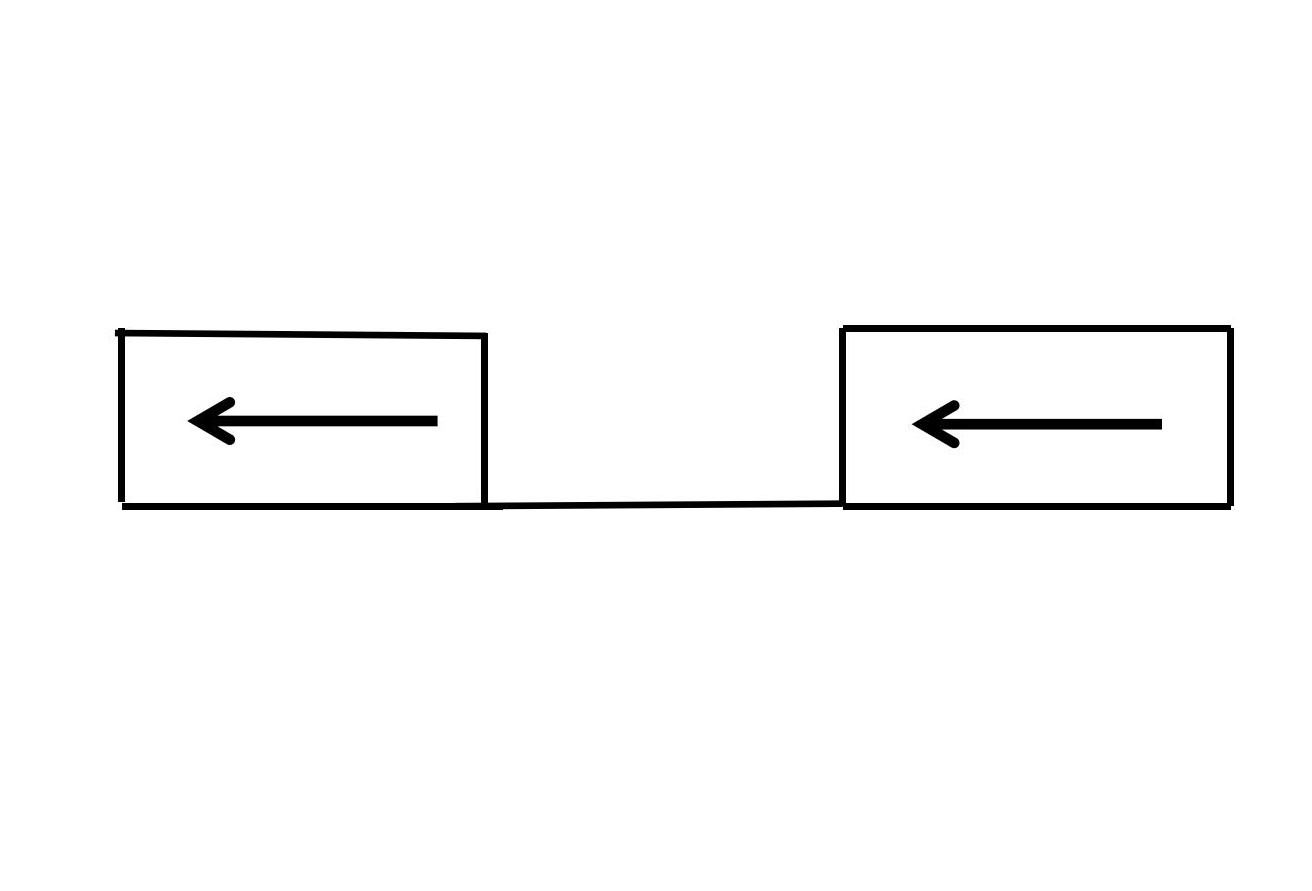
\includegraphics[width=0.95\textwidth]{1}
			\subcaption{平行停车位}
			\label{fig:sample-figure-a}
		\end{minipage}
		\begin{minipage}[c]{0.3\textwidth}
			\centering
			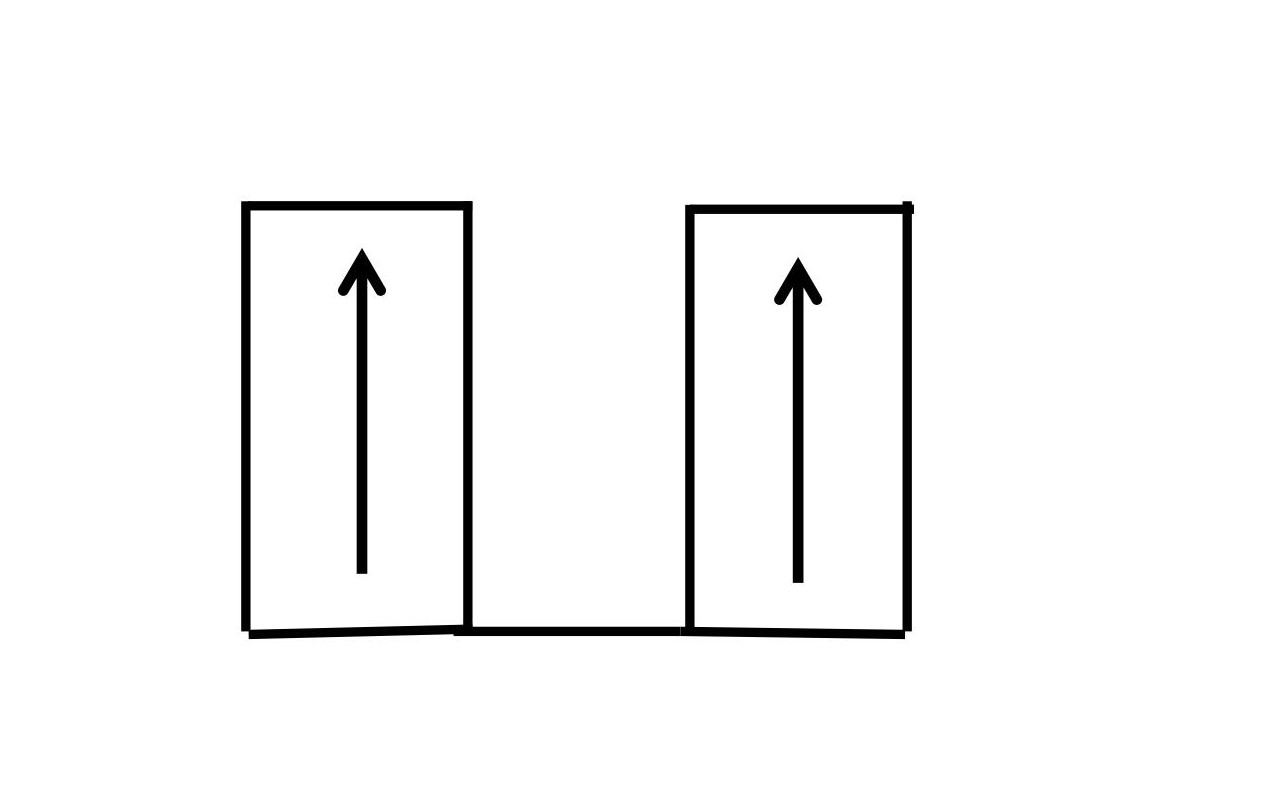
\includegraphics[width=0.95\textwidth]{2}
			\subcaption{垂直停车位}
			\label{fig:sample-figure-b}
		\end{minipage}
		\begin{minipage}[c]{0.3\textwidth}
			\centering
			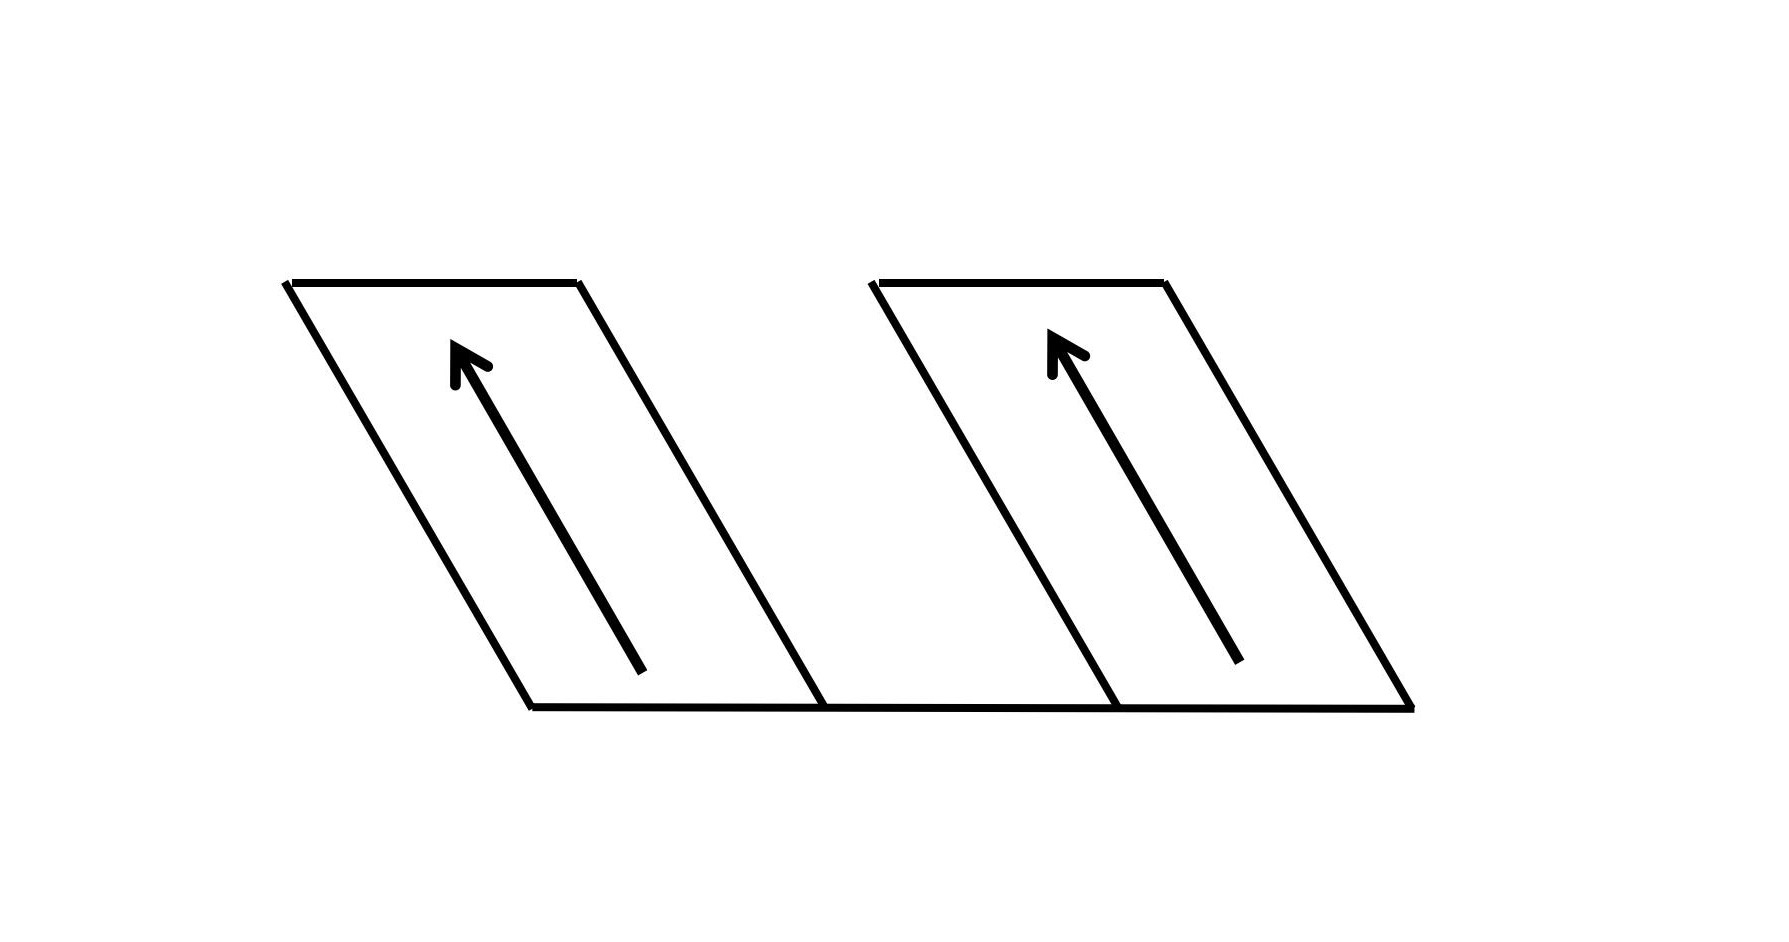
\includegraphics[width=0.95\textwidth]{3}
			\subcaption{倾斜停车位}
			\label{fig:sample-figure-c}
		\end{minipage}
		\caption{三种停车位类型}
		\label{fig:sample-figure}
	\end{figure}
	\subsection{要求的具体问题}
	
	\begin{enumerate}
		\item 问题一
		
		以题目给出的无人车模型的参数,计算车辆最小转弯半径;在限制限制车辆最大加加速度为$20 m/s$的前提下,无人车沿直线行驶时,求解加速到最大限制速度$20km/h$无人车行驶的最短距离;当车速为$20km/h$时,如果无人车从沿直线行驶状态开始转弯,求解路径上的曲率相对路径长度的变化率的取值范围。
		\item 问题二
		
		建立无人车泊车的数学模型,给出从初始位置到指定停车位的泊车轨迹,轨迹应包括  ,绘画出可视化轨迹图(包括每个时刻无人车的行驶路径长度、车辆朝向、速度、加速度、加加速度、角速度、角加速度等信息)。在泊车过程中无人车不能与其发生冲突或碰撞为基础;分别考虑三种不同的车位情况:10 号垂直停车位、82 号平行泊车位、31 号倾斜停车位。
		\item 问题三
		
		在所给的无人车初始位置为前提,以泊车过程中无人车不能与其发生冲突或碰撞为约束,建立泊车模型,计算出最优停车位,并给出从当前位置到停车位的轨迹;。在这个过程中,建立通用模型,使算法能适应车库中任意停车位被占用的状况,并考虑这个过程算法的复杂性。
		\item 问题四
		
		问题四要求我们在假设在当前状态下每小时内从入口进入和从出口离开停车场的车辆均为 30 辆,建立泊车模型,并给出从当前位置到最优停车位的行驶轨迹的仿真结果。此题与问题三不同的是变为一个动态的过程。首先,我们进行时间车辆平均化假定两分钟有一辆车的驶入与离开;其实,以当前车辆为研究对象,讨论车辆的进入和离开对于研究车辆寻找最优车位的影响;最后,基于问题三的算法,对其参数进行改进,求出车位被随机占用和释放的情况下得最优停车位。
	\end{enumerate}

	
	\section{问题分析}
	\subsection{研究现状综述}
	文献[1]中采用一种非完整系统的三步路径规划方法,该方法首先计算无碰撞路径,然后通过考虑非完整约束和其他运动学约束的局部规划器计算的线段连接来逼近第一步中获得的路径,最后将第二步生成的路径更加平滑,但是多步法通常会导致规划出的路径有较多的转折点,这会导致车辆频繁地前进后退。

	文献[2]将平行泊车路径分为两段,采用五次多项式生成路径曲线解决了泊车初始位姿问题,但其第二段曲线也增加了对泊车车位大小的要求。

	总之,现在对于自动泊车轨迹优化或多或少都存在一些不足,相关研究都存在理论层面,缺乏经验支撑,有待完善。

	

	\subsection{对问题的总体分析和解题思路}

	题目可以看作是一个约束条件和目标的路径规划问题,其中的技术关键有:三种停车位泊车最优泊车轨迹规划、约束条件的选取、最短路径的规划。该问题一个考虑对车辆的碰撞约束、转向性能约束和几何关系约束。在模型在满足约束条件的前提下尽可能满足:1.在最短时间内寻找到最优停车位;2.在泊车的过程中确保安全;3.算法较高的求解率与降低算法的复杂度。
	
	\begin{figure}[h]
		\centering
		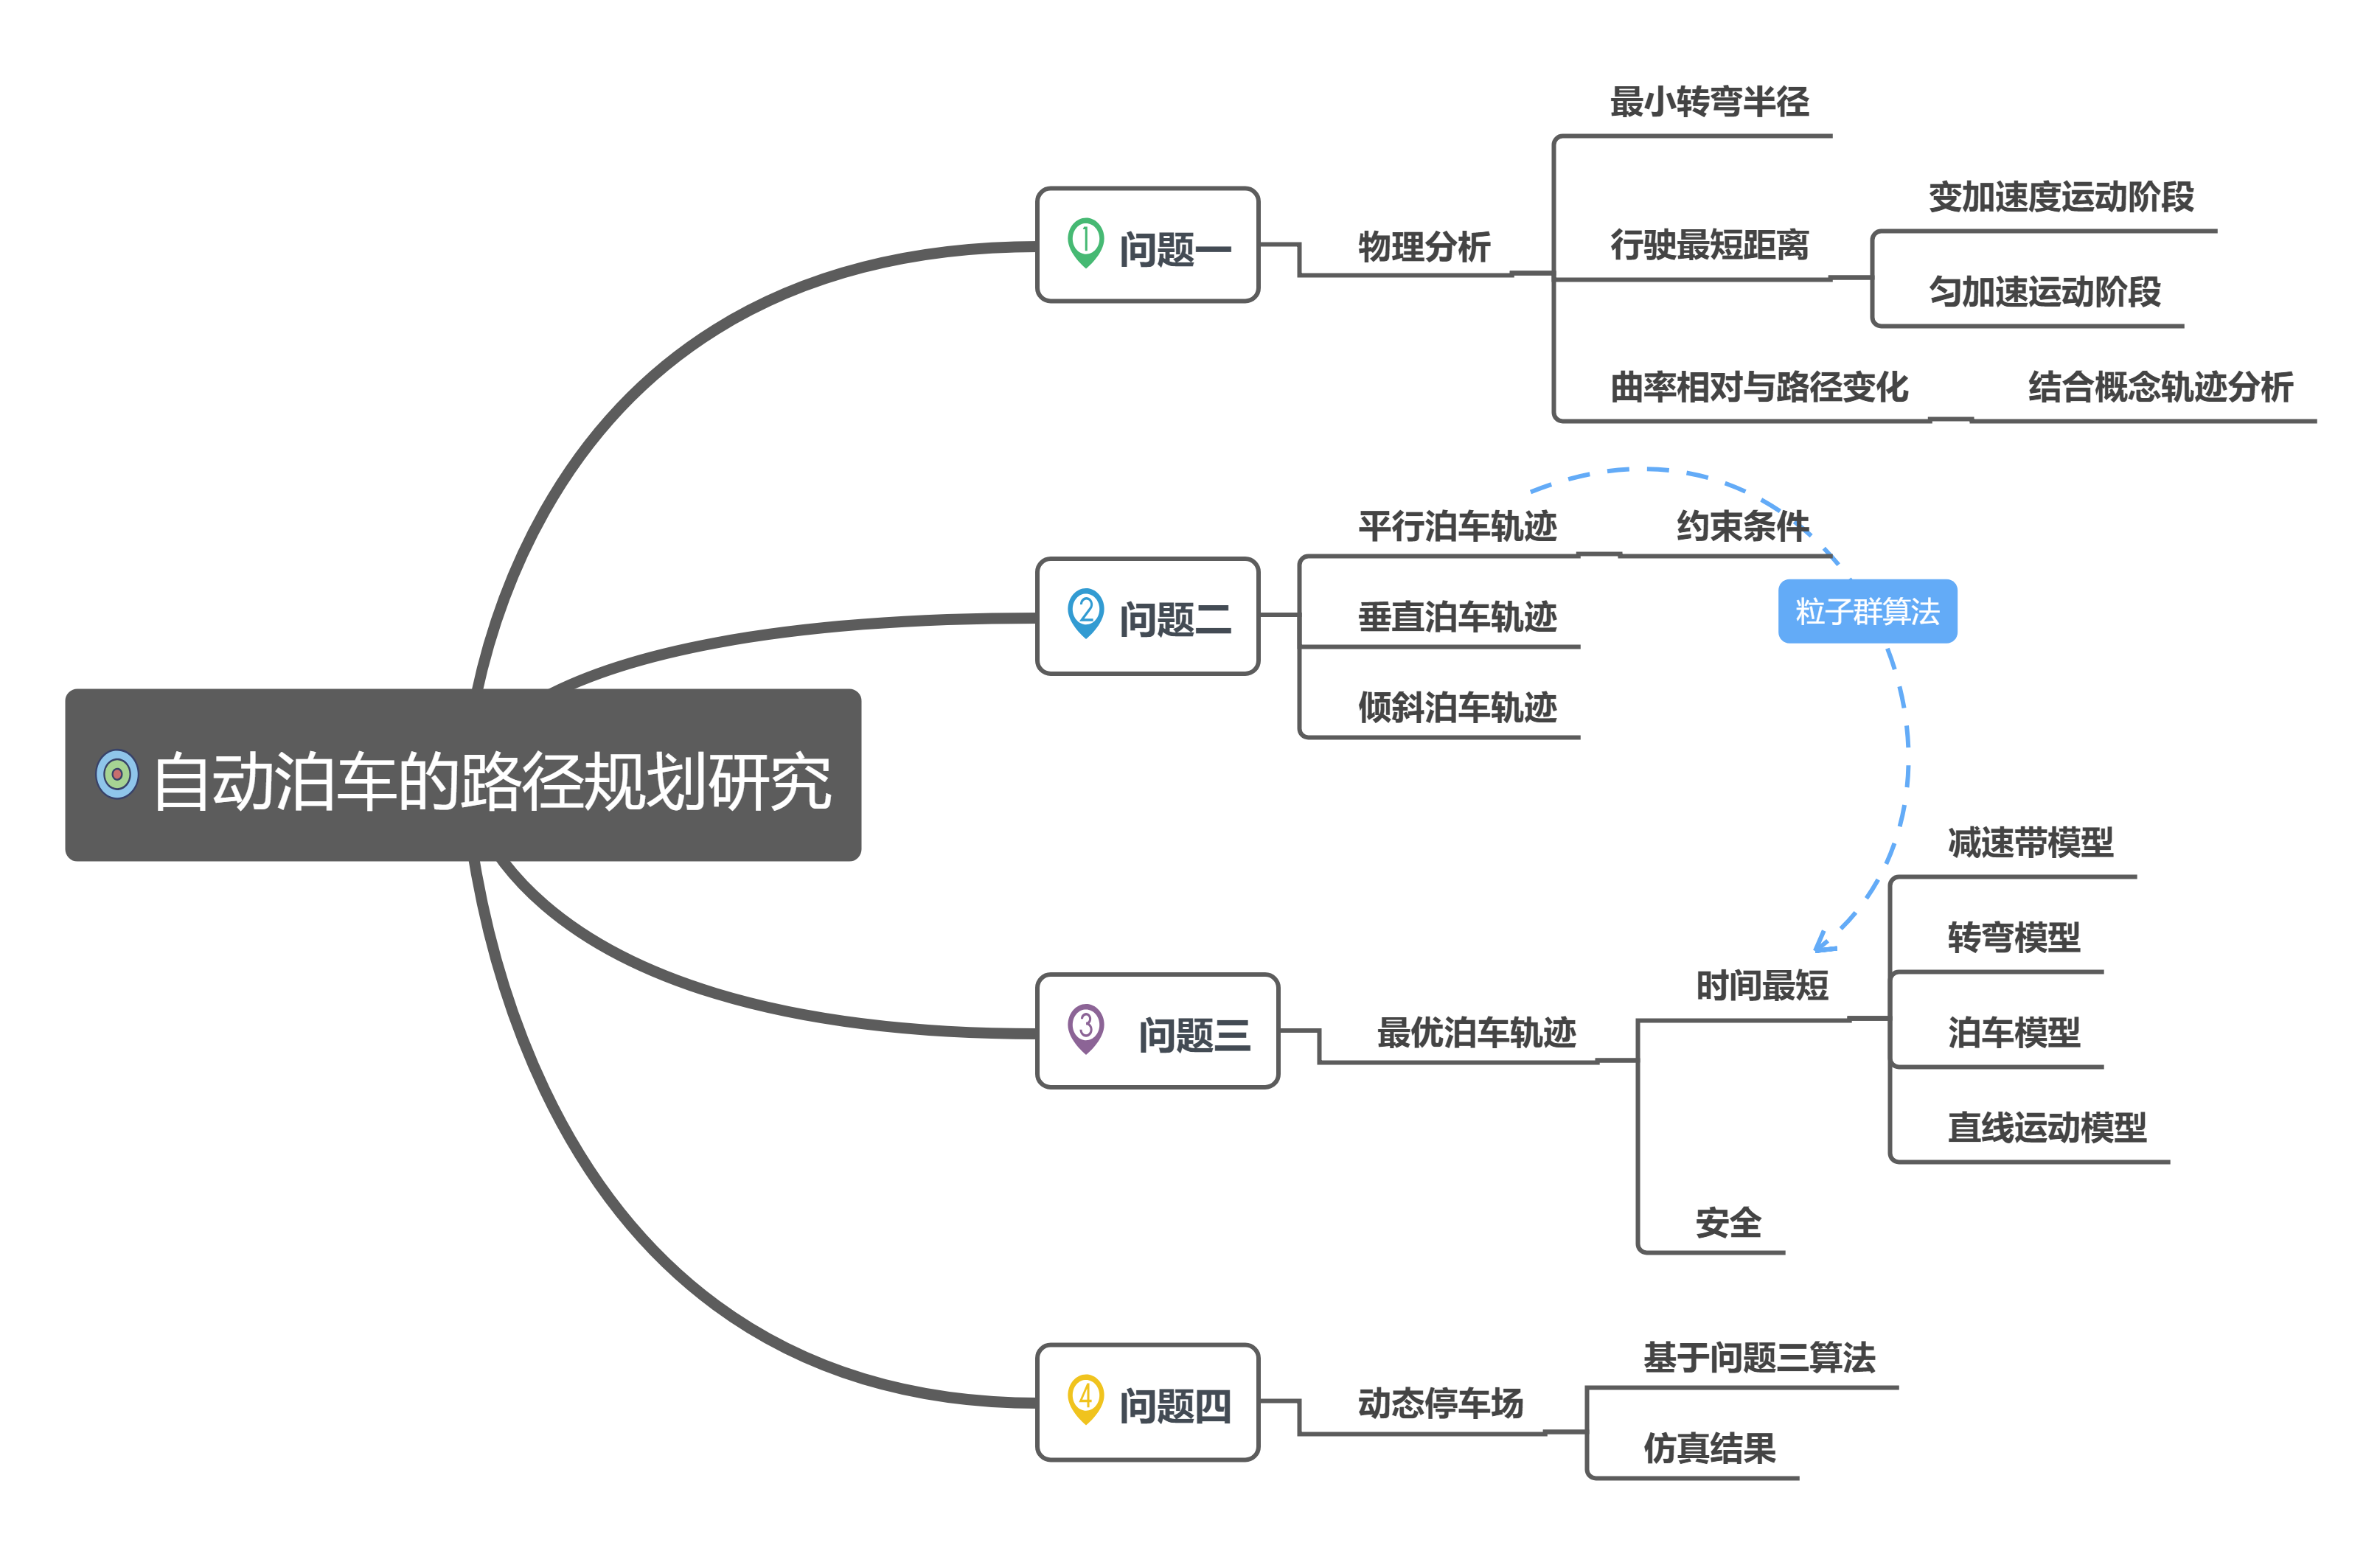
\includegraphics[width=.9\textwidth]{思维导图}
		\caption{自动泊车路径规划建模整体思路}
		\label{fig:circuit-diagram}
	\end{figure}

	\subsection{问题的具体分析和对策}

	\subsubsection{对问题一的分析}

	问题一要求我们研究最小转弯半径,在加速度与加加速度限制下加速到最大限制速度$20km/h$最短需要行驶多少距离,以及车辆由直线变为转弯时路径上的曲率相对路径长度的变化率的取值范围三个小题。通过分析,这三个小题均属于物理题目,无需编程只需要推理出公式即可解出答案。

	第一小题:推导出车辆转弯时的最小转弯半径,代入题目所给的无人车参数,即可解出值。

	第二小题:为了得到行驶的最短路径,将此过程分为变加速直线运动阶段和匀加速直线运动阶段,分别求出两个阶段的行驶路径表达式,在对两个阶段距离求和,即可得到结果。

	第三小题:从直线行驶变为转弯过程中,我们研究从即将转弯到方向盘打满这一阶段的曲率变化率,依据题目所给的方向盘转速和方向盘最大转角,可以分析出这一阶段的时间,进而求出这阶段的行驶路程。在方向盘打满时,车轮转角最大,此时对应最大曲率,直线行驶时对应的曲率为零。进而可以求出这一阶段的曲率相对于路径的变化率最大值。
	\subsubsection{对问题二的分析}

	问题二要求我们建立无人车泊车的数学模型,给出从初始位置到指定停车位的可视化轨迹图,在泊车过程中无人车不能与其发生冲突或碰撞为基础绘画出10 号垂直停车位、82 号平行泊车位、31 号倾斜停车位的泊车轨迹。本题的重点在于最优三种泊车情况的轨迹规划,因为驶入车库跟驶出车库是一个可逆的过程,为此我们提出一种逆泊车的概念,规划出一条从高约束区的车库内行驶进低约束区的车库外,在通过逆变换得到泊车轨迹。其次通过轨迹参数组合取值范围得出所有可行的泊车轨迹,最后结合考虑碰撞约束、转向性能约束和几何关系约束,利用粒子群算法得出最优泊车轨迹。
	\subsubsection{对问题三的分析}

	问题三要求我们根据当前的停车位状况,建立泊车模型,寻找到最优停车位,并要求建立通用模型使之能够适应任意车位被占用的情况。最优停车位的目标为安全情况下泊车过程最短时间;我们将整个停车时间分为四个时间段考虑,分别为直线加速路程时间、转弯时间、减速带减速时间和泊车时间,根据可用车位的具体位置考虑泊车总时间由哪些时间段组成。最后,利用设计模拟停车位被随意占用的算法,并且考虑其算法的复杂程度。
	\subsubsection{对问题四的分析}
	
	问题四要求我们在假设在当前状态下每小时内从入口进入和从出口离开停车场的车辆均为 30 辆,建立泊车模型,并给出从当前位置到最优停车位的行驶轨迹的仿真结果。此题与问题三不同的是变为一个动态的过程。首先,我们进行时间车辆平均化假定两分钟有一辆车的驶入与离开;其次,以当前车辆为研究对象,讨论车辆的进入和离开对于研究车辆寻找最优车位的影响;最后,基于问题三的算法,对算法进行补充完善,求出车位被随机占用和释放的情况下得最优停车位。
	\section{模型假设}
	\begin{enumerate}
		\item 假设无人车控制点位于后轴中心上,速度方向与轨迹点的车身方位角相等;
		\item 假设在自动泊车过程中没有发生两车相撞;
		\item 轮胎与地面的摩擦消耗的时间忽略不计;
	\end{enumerate}
	
	\section{名词解释与符号说明}
	\subsection{名词解释}
	\begin{enumerate}
		\item 逆泊车轨迹:泊车过程是一个从低约束区的车库外行驶进高约束区的车库内的过程,因为驶入车库跟驶出车库是一个可逆的过程,所以下文提出逆泊车轨迹,规划出一条从高约束区的车库内行驶进低约束区的车库外,在通过逆变换得到泊车轨迹。
		\item 阿克曼结构:汽车在直线或者转弯两个行驶过程中,四个车轮的运动轨迹必须符合他的自然运动轨迹,从而保证轮胎与地面始终处于纯滚动,并且四个车轮的轴线都互相平行。
		\item 控制点:位于无人车车身称轴上的一点,基于题目所给的阿克曼转向模型,本研究假设控制点位于后轴中心上。在行驶过程中,控制点的位置会与轨迹点相重合,而且控制点处的速度方向将与轨迹点的方向角一致。
		
	\end{enumerate}

	\subsection{符号说明}
	\begin{table}[htbp]
		\centering
		\caption{(注:此为本文的主要符号说明,其它符号解释详见正文部分)} \label{fig:aa}
		\renewcommand\arraystretch{0.75}{
		\setlength{\tabcolsep}{5mm}{
			\begin{footnotesize}
		\begin{tabular}{ccc}
		\Xhline{0.08em}
		符号 & 符号说明&单位 \\
		\Xhline{0.05em}
		$L$ & 车子轴距 & $m$\\
		$W$ & 车间距&$m$\\
		$L_{f}$ & 车长&$m$\\
		$L_{W}$ & 车宽&$m$\\
		$\delta_0$ & 前轮转角&$^{\circ}$\\
		$\theta$ & 车身方位角&$^{\circ}$\\
		$L_p$ & 车库长度& $m$\\
		$W_p$ & 车库宽度&$m$\\
		$\varepsilon$ & 车库安全距离&$m$\\
		$a$ & 车辆加速度&$m/s^2$\\
		
		\Xhline{0.08em}\\
		\end{tabular}
	\end{footnotesize}
		}}
	  \end{table}

	\section{模型的建立与求解}
	\subsection{问题一模型的建立与求解}
	\subsubsection{模型的建立}
	\begin{enumerate}
		\item 阿克曼车辆模型 
		
		本文的无人车采用阿克曼结构,前轮转向后轮驱动,相较于传统的单铰链转向技术相比,虽然两者都能使内外转向轮在转动时路径指向同一个圆心,但是阿克曼转向技术能有效避免单铰链转向技术的缺点,具体表现为阿克曼结构能够克服在转弯过度时车轮容易卡死而动不了。阿克曼结构在无人车转弯的时候,内外车轮转过的角度不一样,内轮转弯半径要小于外轮的转弯半径,使得四个车轮路径圆心会相交于后轴的延长线上瞬时转向中心,让车辆可以顺畅的转弯,如图3。
		\begin{figure}[h]
			\centering
			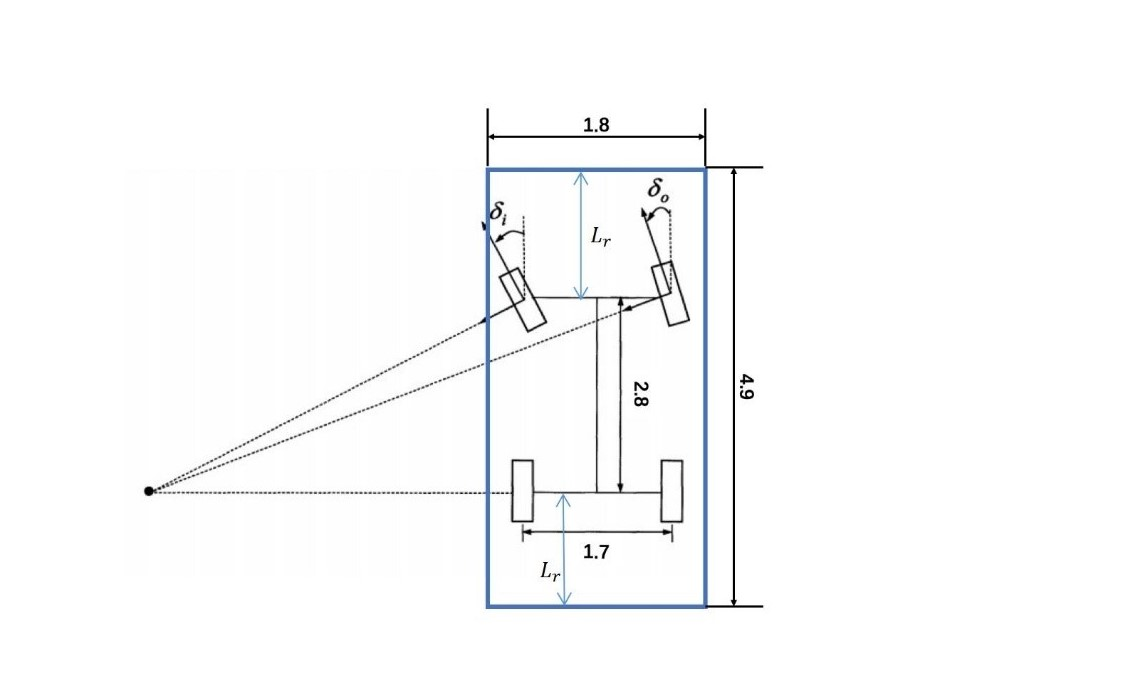
\includegraphics[width=.6\textwidth]{4}
			\caption{阿克曼车辆模型车辆}
			\label{fig:circuit-diagram}
		\end{figure}
		
		阿克曼结构无人车具体参数如下:
		\begin{table*}[htbp]
			\centering
			\caption{阿克曼结构无人车参数} \label{fig:aa}
			\renewcommand\arraystretch{1.5}{
			\setlength{\tabcolsep}{1mm}{
			 \begin{footnotesize}
			\begin{tabular}{ccccccc
				ccc}
			\hline
			\textbf{名称}	&车长&车宽&车子轴距&轮间距&最大油门加速度&加加速度&方向盘最大转角&方向盘最大转速&极限最大减速度\\
			\hline
			\textbf{数值}   &$4.9m$&$1.8m$&$2.8m$&$1.7m$&$3.0m/s^{2}$&$20.0m/s$&$470^{\circ}$&$400^{\circ}$&$-6.0m/s^{2}$\\
			\hline
			\end{tabular}
			\end{footnotesize}}}
			
		
		  \end{table*}
	
		  根据题目所给的已知条件,方向盘最大转角为$470^{\circ}$,方向盘UI前轮转角的传动比为$16:1$,即方向盘每转动$16^{\circ}$,前轮转动$1^{\circ}$,因此可得前轮最大转角为$\delta_{0max}=470^{\circ}\frac16=29.375^{\circ}$。
	
	此外,根据题目给定的阿克曼车辆模型,可认为其为对称结构,前轮车轴距离车辆前端的距离与后轮车轴距离车辆后端的距离相等,即车辆前悬长和后悬长相等,从而求得悬长$L_r=1.05m$。
	

	\end{enumerate}

	

	\subsubsection{模型的求解}
	\begin{enumerate}
		\item 车辆最小转弯半径

		车辆最小转弯半径指的是当转向盘转到极限位置,汽车回转时汽车的前轮外侧循圆曲线行走轨迹的半径。此物理量在很大程度上表征了汽车能够通过狭窄弯曲地带或绕过不可越过的障碍物的能力,转弯半径越小,汽车的机动性能越好。下面将对无人车最小转弯路径示意图进行分析,示意图见图4.
		\begin{figure}[H]
			\centering
			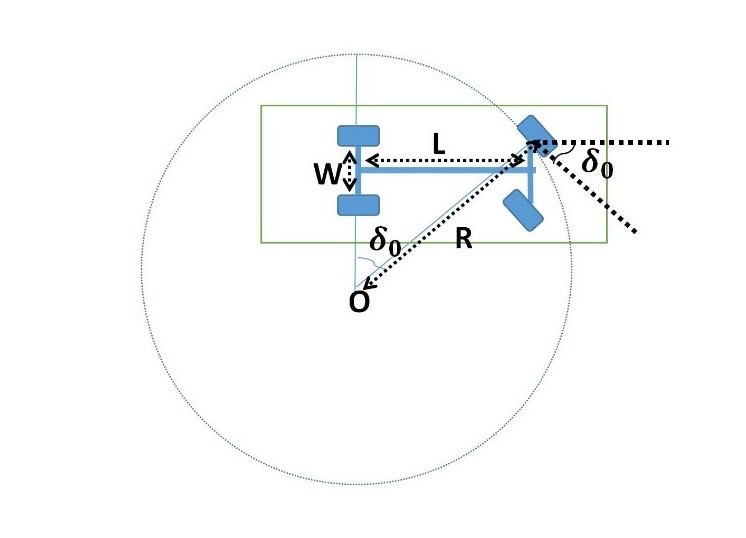
\includegraphics[width=.6\textwidth]{5}
			\caption{无人车最小转弯半径示意图}
			\label{fig:circuit-diagram}
		\end{figure}
		
		基于阿克曼车辆结构在转弯时内外转向轮在转动时路径指向同一个圆心,并且四个车轮路径圆心会相交于后轴的延长线上瞬时转向中心的特点,在方向盘转到最大角度时,外侧转弯轮转角最大,即$\delta_{0max}$为$29.375^{\circ}$,此时的转弯半径最小。
		
		由图4可以分析得到如下公式:
		\begin{equation}
		R_{min}=\frac{L}{sin\delta_{0max}}
		\end{equation}
		式中L为无人车车子轴距;$R_{min}$为最小转弯半径;$\delta_{0max}$为前外侧轮最大转弯角。将题目所给的无人车模型参数代入(1)式中,可得$R_{min}=5.70m$。
		\item 加速过程行驶的最短距离
	
		无人车以最大加加速度为$20 m/s$沿直线行驶时,加速到最大限制速度$20km/h$,此运动过程分为两个运动阶段:
			  \begin{itemize}
				  \item [$step1$]变加速直线运动阶段
				  
				  以$20 m/s$的加加速度加速到加速度为$3 m/s$过程中,行驶的距离记为$S_{1}$,计算公式如下:
				  
				  \begin{equation}
					a=a_0+\alpha t
				  \end{equation}
				  \begin{equation}
					v=\int_{0}^{t}{a\ dt=v_0+}a_0t+\frac{{1}}{2}\alpha t^2
				  \end{equation}
				  \begin{equation}
					S_1=\int_{0}^{t}{v\ dt=v_0t+\frac{{1}}{2}a_0t^2+}\frac{1}{6}\ \alpha t^3
				  \end{equation}
				  式中:为油门加加速度;为加速度;为行驶时间, 为初始加速度,为初始速度。
				  
				  将题目中所给的已知物理量代入式(2)$\sim$ (4)中,求解出$t$,$v_1$,$S_1$。
				  \item [$step2$]匀加速直线运动阶段
				  
				  以加速度为$3 m/s$做匀加速直线运动加速至最大限制速度20km/h过程中行驶的距离,记为,计算公式如下:
				  
				  \begin{equation}
					S_2=\frac{v_2^2-v_1^2}{2a_1}
				  \end{equation}
				 
				  式中:为最大限制速度;为该阶段的初始速度,为该阶段的加速度,即油门的限制加速度。


				  综上所诉,可以求得题目需求的加速过程中的最短行驶距离$S={S_1+S}_2$。计算过程:假设车辆从静止开始运动,则$a_0=0$,$v_0=0$。根据已知条件并联立式(2)$\sim$ (4),解得:$t_1=0.15s$, ${\ v}_1=0.225m/s$, $S_1 =0.01125m$, $S_2=5.1356m$。因此加速过程中行驶的最短距离为$S=5.2481m$。

			  \end{itemize}
		\item 曲率相对于路径变化率取值范围
	
		曲线的曲率就是针对曲线上某个点的切线方向角对弧长的转动率,通过微分来定义,表明曲线偏离直线的程度。曲率越大,表示曲线的弯曲程度越大,曲率的倒数就是曲率半径。汽车在转弯时可大致分为三个阶段:(1)打方向盘阶段,以最大方向盘转速打方向直到打满。(2)第二阶段以最大车轮转角作圆周运动。(3)回正方向盘。按照一般的习惯,回正方向盘时车头已经转过$90^{\circ}$,所以此阶段可不予考虑。在第一阶段中,随着方向盘转角越大,对应的转弯半径也越小,因此在转弯过程中,行驶轨迹为一条曲线。车辆在转弯过程中前外轮轨迹示意图如图5所示:
		\begin{figure}[h]
			\centering
			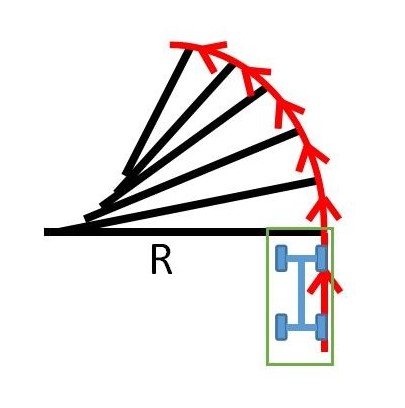
\includegraphics[width=.3\textwidth]{6}
			\caption{汽车转弯前外轮轨迹示意图}
			\label{fig:circuit-diagram}
		\end{figure}
		
		由曲率的定义可知曲率的计算公式为:

		\begin{eqnarray}
			k=\frac{d\theta}{ds}=\frac{1}{R}
		\end{eqnarray}
		式中表示曲线上两端点切线方向角的转角,$ds$表示两点间的距离。转弯前车速为$20km/h$,即$5.56m/s$,转弯的过程可视为匀速运动。第一阶段的时间记为$t_1$,由题意知$t_1=470/400 =1.175s$,所以该阶段走过的路程$s=vt_1=6.53m$。车从直线运动状态开始转弯,故起始曲率$k_0=0$,由(1)式知$R_{min}=5.70m$。当方向盘打满时,前外轮转弯角达到最大值,此时转弯半径取得最小值,考虑到一般车轮轮胎宽度为$d_1=0.215m$以及无人车轮胎与车身对称轴为$l_1=1m$,故控制点到圆心距离$R_{Kmax}=R_{max}-l_1+d_1=4.915$,此时控制点最大曲率为0.203。所以曲率相对于路径的变化率限制的限制为$[0,0.031]$。
	\end{enumerate}


	\subsection{问题二模型的建立与求解}
	\subsubsection{模型的建立}
	\begin{enumerate}
		\item 车辆运动学模型的建立
		
		为了方便下文对于无人车自动泊车的路径规划和路径跟踪控制的研究展开,需要先建立车辆运动学模型,在整个自动泊车过程,无人车往往处于低速行驶的状态,并且车轮处于大转角状态。在低速状态研究下,轮胎所受的侧偏力往往可以忽略。由于行驶过程中轮胎没有发生滑移,其转向轴线均交于一点作圆周运动。因此我们小组将整车视为一个刚体,从而采用阿克曼转向原理来进行运动学研究。

		模型如图6所示,$P$点为后轴中心点,即题目所假设的控制点,控制点的位置会与轨迹点相重合,控制点处的速度方向$V$将与轨迹点的方向角一致;汽车的四个顶点分别为$A(x_A,y_A)$,$ B(x_B,y_B)$, $C(x_C,y_C)$,$ D(x_D,y_D)$\cite{label3}。

		\begin{figure}[H]
			\centering
			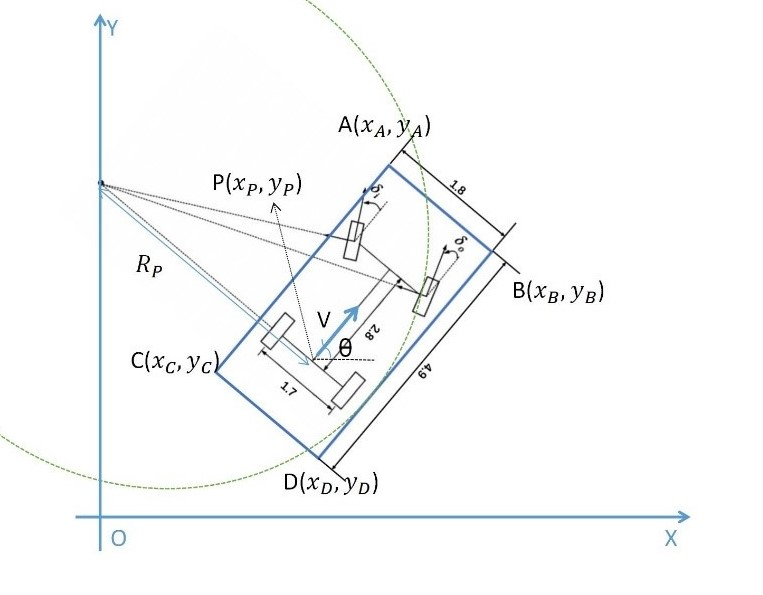
\includegraphics[width=.45\textwidth]{7}
			\caption{车辆运动学模型}
			\label{fig:circuit-diagram}
		\end{figure}
		根据上图的几何关系,在笛卡尔坐标系下,其运动学方程可表示为:

		\begin{equation}
			\left\{\begin{matrix}
				\dot{x_P}=Vcos\theta
				\\ \dot{y_P}=Vsin\theta
				\\ \theta=\frac{V}{L}tan\delta_0
				\end{matrix}\right.
		\end{equation}

		上式中:$V$为后轴控制点的速度;$\theta$为车身方位角;$\delta_0$前轴外轮等效转角。
	
		将式(9)$\sim$(10)以$T$周期进行离散化可得到如下的离散化模型,即第$k+1$个周期可以由第$k$个周期离散点参数进行表示:
		\begin{equation}
			\left\{\begin{matrix}
				x\left(k+1\right)=x\left(k\right)+T\cdot cos\theta\left(k\right)\cdot v\left(k\right)
			   \\ y\left(k+1\right)=y\left(k\right)+T\cdot sin\theta\left(k\right)\cdot v\left(k\right)
			   \\ \theta\left(k+1\right)=\theta\left(k\right)+T\cdot cos\theta\left(k\right)\cdot v\left(k\right)
			   \\ \delta_0\left(k+1\right)=\delta_0\left(k\right)+T\cdot\delta_0
			   \\ v\left(k+1\right)=v\left(k\right)+T\cdot a\hfill
			   \end{matrix}\right.
		\end{equation}
		下文将基于此车辆运动学模型建立平行泊车车库模型。
		\item 车辆转弯模型
		
		在停车场内涉及到多个转弯问题,因此对停车场入口第一个转弯建立模型进行分析,其他的路口转弯模型也与之等效。
		
		在整个自动泊车的过程中,就行驶轨迹而言,希望尽可能的保持平滑,其中需要考虑的一点是使轨迹的曲率变化率尽可能小,则有如下规划目标:即需要各轨迹点曲率变化率的绝对值的平均值尽可能小。而圆弧的曲率变化率始终为 0,因此,无人车转弯路径规划为四分之一的圆弧。
		
		安全泊车是自动泊车过程的核心问题之一,因此需要考虑无人车在转弯时与转弯区域安全边界的问题。边界为在无人车转弯的过程中,需要考虑两种边界触碰问题:其一为无人车转弯时汽车右侧碰撞到拐角$A$点,另一为在转弯过程即将结束时触碰到道路上边界的一点B。在本题中小组假设最小安全距离$d_{min}=0.3$,在$A$、$B$两点处分别作半径为$0.3m$的圆 $A$ 和圆 $B$,规定当车身进入圆 $A $或圆$ B$,则说明规划的轨迹不安全;而当车身刚好与圆 $A$ 或圆 $B $相切或相离时,则说明轨迹安全。示意图见图7。
		
		\begin{figure}[h]
			\centering
			\begin{minipage}[c]{0.4\textwidth}
				\centering
				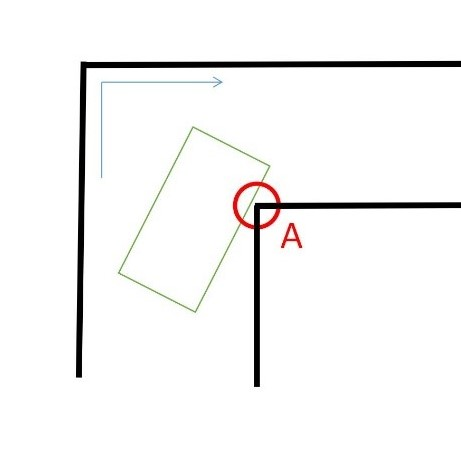
\includegraphics[width=0.95\textwidth]{8}
				% \subcaption{平行停车位}
				\label{fig:sample-figure-a}
			\end{minipage}
			\begin{minipage}[c]{0.4\textwidth}
				\centering
				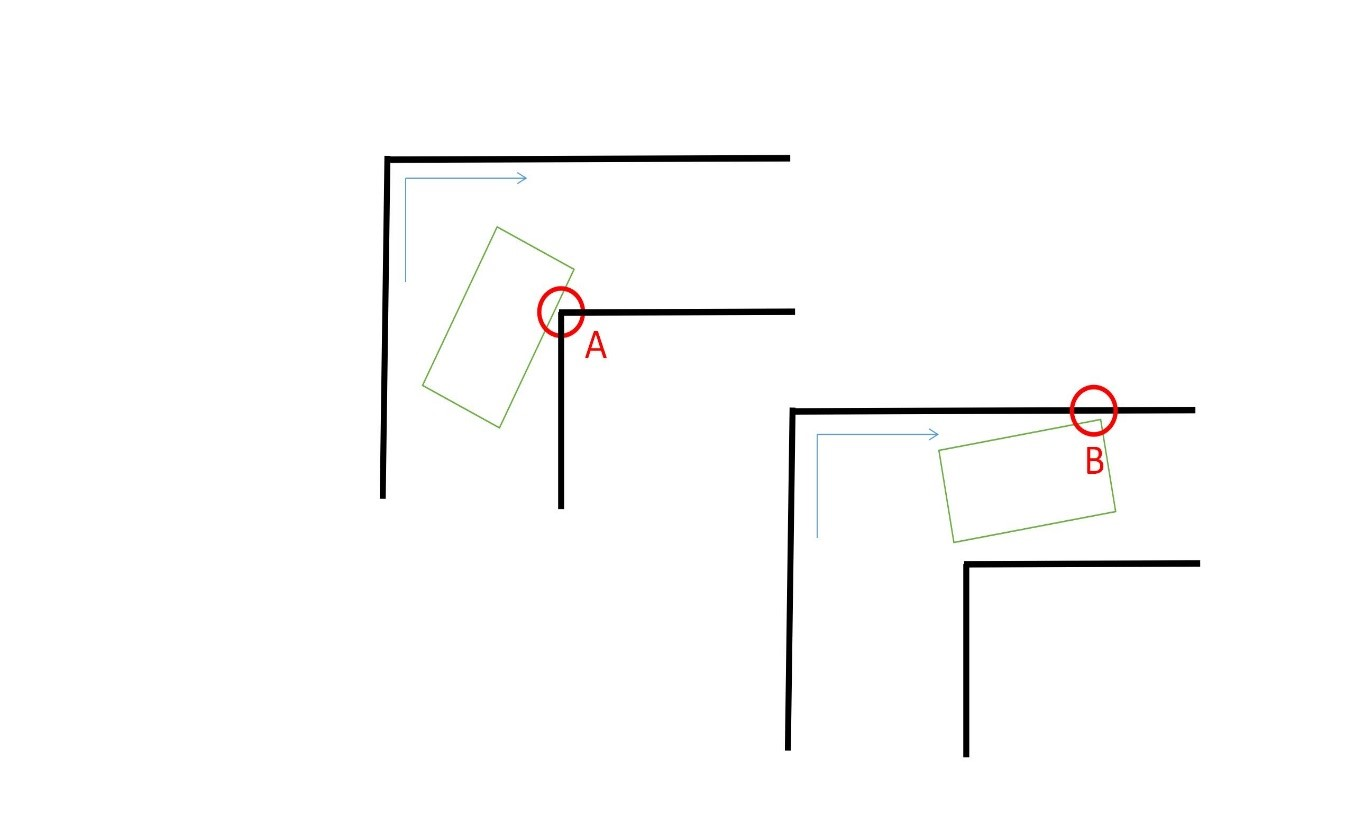
\includegraphics[width=0.95\textwidth]{9}
				% \subcaption{倾斜停车位}
				\label{fig:sample-figure-c}
			\end{minipage}
			\caption{无人车路口转弯碰撞示意图}
			\label{fig:sample-figure}
		\end{figure}

		为了简化下文的研究,假设无人车转弯时做匀速圆周运动,并且假定后轴中心点,即控制点,处于道路的中心,在无人车车头距离第一个垂直型停车位上边$2.4m$的时候,开始做匀速圆周运动,因此只需讨论此情况转弯是否会触碰到转弯区域的安全边界,转弯示意图见图8 。
		
		\begin{figure}[H]
			\centering
			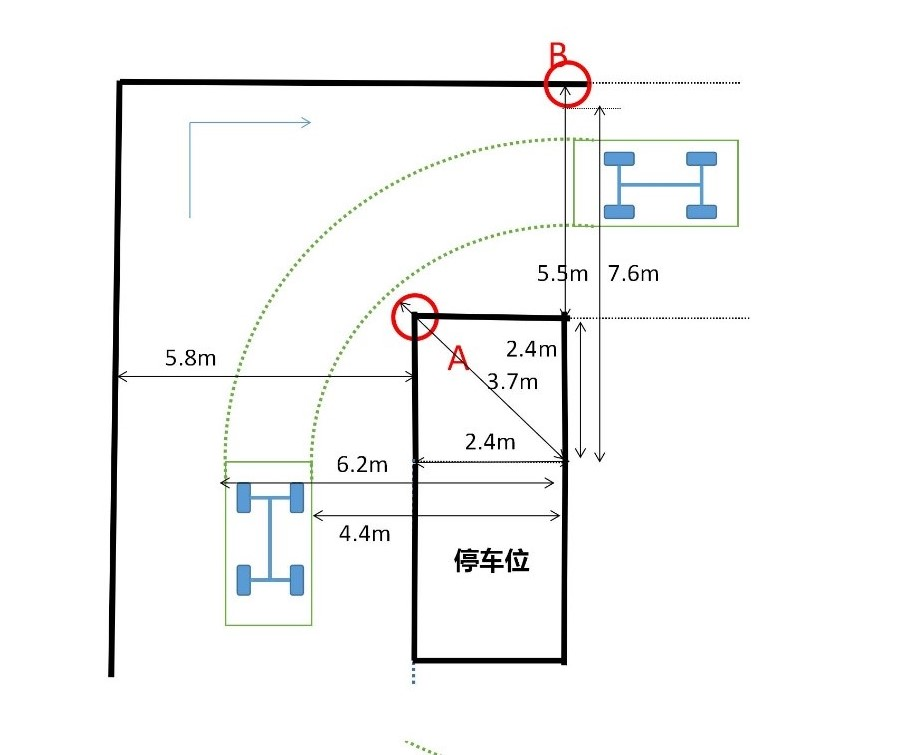
\includegraphics[width=.5\textwidth]{10}
			\caption{无人车转弯示意图}
			\label{fig:circuit-diagram}
		\end{figure}

		依上图知,当车身右侧转弯半径小于不碰撞拐角A所要求的最大半径$3.7m$,或者车身左侧半径小于不触碰到边界B所要求的最小半径$7.6m$,此时无人车可以安全转弯。按照假设条件,可知无人车转弯时车身右侧与车身左侧所作的轨迹为半径$4.4m$和$6.2m$的圆,满足安全边界条件可以顺利转弯。
	
		\item 泊车轨迹规划
		
		\begin{enumerate}
			\item 82号平行泊车轨迹规划
	
	泊车过程是一个从低约束区的车库外行驶进高约束的车库内的过程,但是驶入车库跟驶出车库是一个可逆的过程,因此为了能够极大简化问题,本文提出一种逆泊车轨迹以下文提出逆泊车轨迹,规划出一条从高约束区的车库内行驶进低约束区的车库外,在通过逆变换得到泊车轨迹\cite{label4}。

	本文设定无人车的控制点在车轮后轴中心点,并且车辆所停的位置处于车库的中间位置,当无人车控制点在初始位置P1时,车辆轮廓CD与车库左边界存在一个安全距离$\varepsilon$。此时,依据平行泊车轨迹规划过程分析,见图9,停放点位置P1的位置坐标为$P1(x_p,y_p)=(L_r+\varepsilon,{Wp-\varepsilon}/frac2)$,当车库的参数与安全距离确定时,该停车点P1的位置就随之确定。


	\begin{figure}[H]
		\centering
		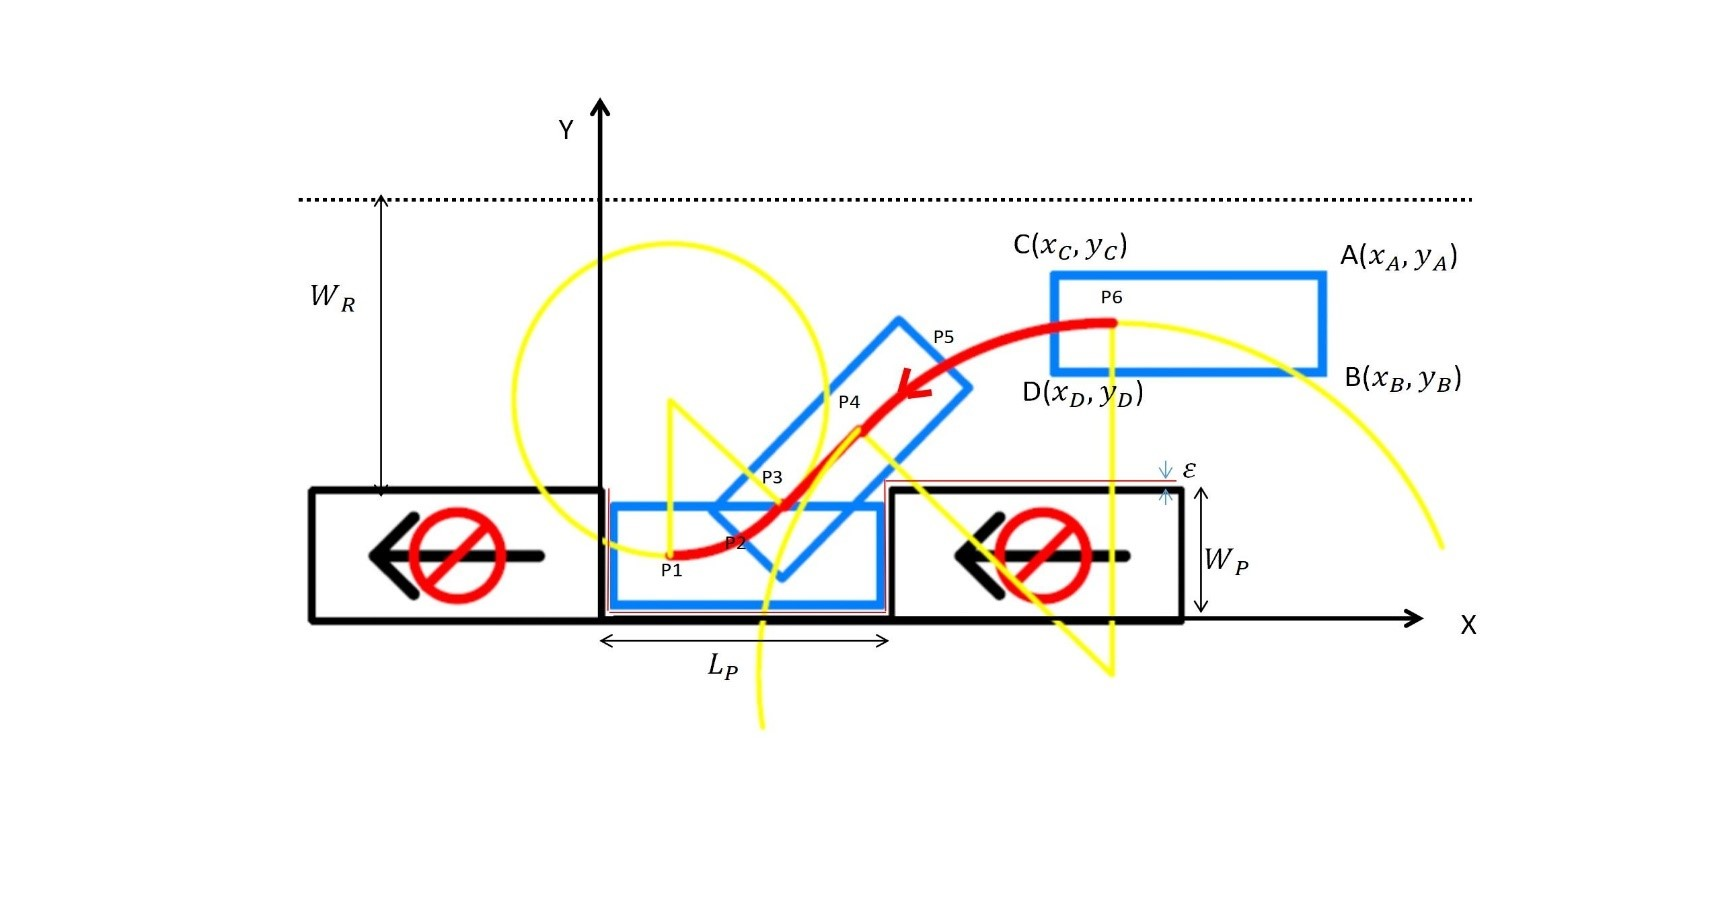
\includegraphics[width=.8\textwidth]{11}
		\caption{平行泊车轨迹规划过程分析}
		\label{fig:circuit-diagram}
	\end{figure}

	对于车辆而言,当给定速度与转角时,车辆将会产生相应的位移,此时车辆的行驶轨迹的曲率是连续的,但是如果在行驶的过程中突然停车转向,那么停车前后的轨迹的曲率将发生突变。本文利用这一特点设计了曲率连续变化的轨迹。

	根据泊车经验,对于车辆从车库内行驶出车库外的过程,本文对逆向平行泊车轨迹规划的过程为:以车轮后轴中心为研究点,P1为起始点,在P1点时的初始速度和车身方位角均为0,在P1至P2段对应的时间段里,方向盘以某一个均匀速率转至某一角度,此角度小于$\delta_{0max}$,对应的前轮转向角的变化为图中P1至P2段,但是在实际的泊车过程中,车辆应是从P2点行驶至P1点,等效前轮转向角也应是从P2点对应的$\delta_0$变化至0;P2至P6段的转角变化过程原理亦是如此。

	\begin{equation}
		\left\{\begin{matrix}
			t_{P1-P2}=t_{P5-P6}=0.5t_{P3-P4}=\frac{\delta_0}{\delta_{0max}}
			\\ t_{p2-p3}=t_1
			\\ t_{P4-P5}=t_2
			\end{matrix}\right.
	\end{equation}

	在无人车自动泊车过程中,要确保安全泊车,即无人车不能与其发生冲突或碰撞,因此需要满足的避碰条件和转向性能约束有:
	\begin{enumerate}
		\item 碰撞约束:
		\begin{itemize}
			\item 车辆外边缘左前顶点$A(x_A,y_A)$应避免与道路边界碰撞;
			\item 车辆外边缘右前顶点$B(x_B,y_B)$应避免与泊车位右边界上顶点发生碰撞;
			\item 车辆外边缘右后顶点$D(x_D,y_D)$应避免与泊车位下边界上顶点发生碰撞;
		\end{itemize}
		\item 转向性能约束:前轮转向角应不超过车辆最大转角值;
		\item 几何关系约束:车辆行驶过车中任意一点左边可由后轴中心坐标和车辆车身方位角通过几何表示;
	\end{enumerate}

	\begin{figure}[H]
		\centering
		\begin{minipage}[c]{0.3\textwidth}
			\centering
			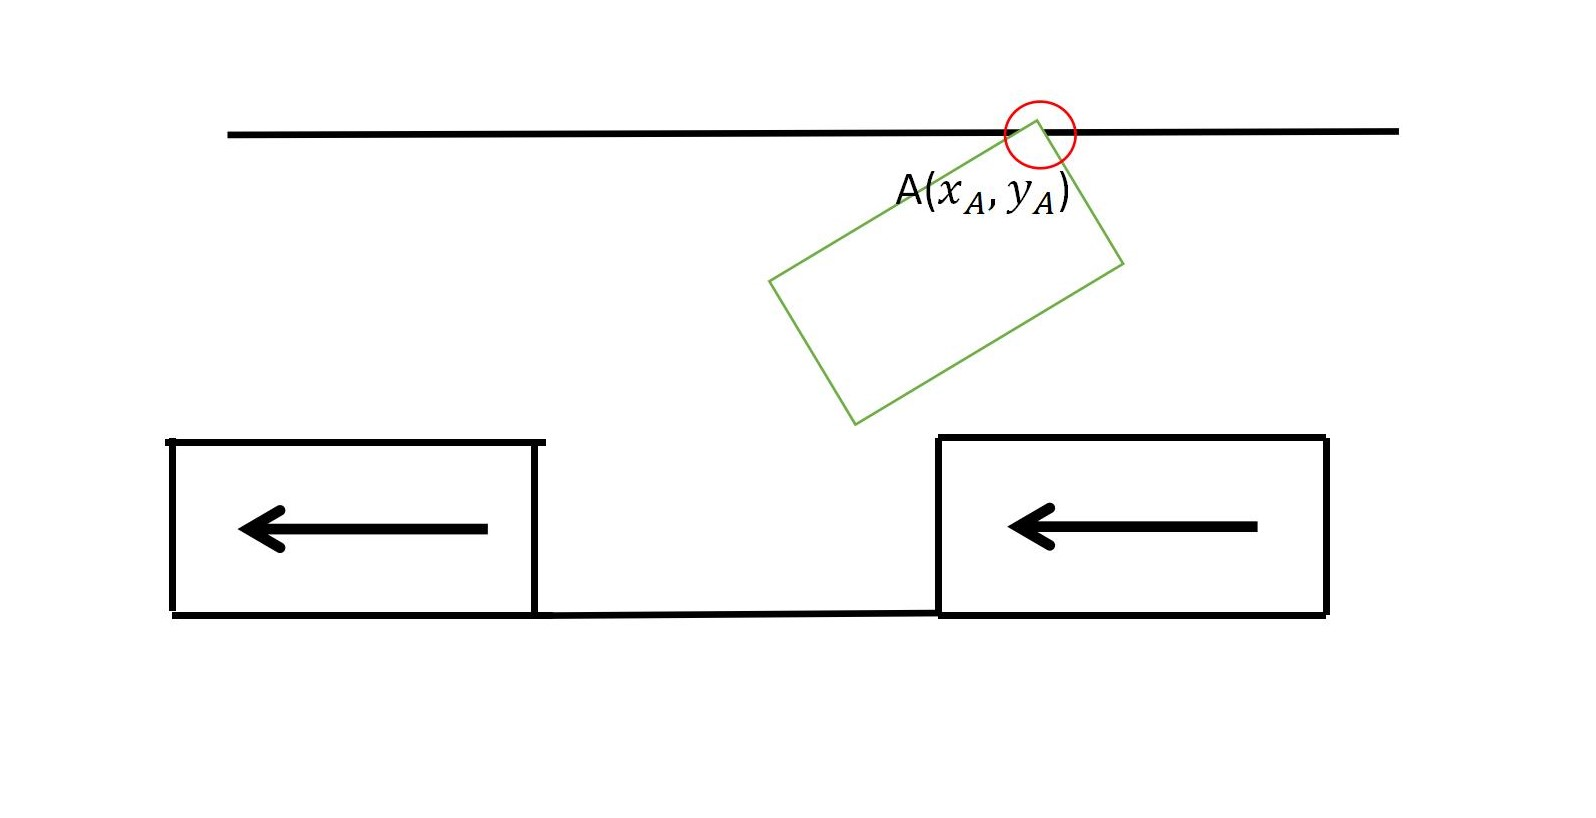
\includegraphics[width=1\textwidth]{12}
			% \subcaption{平行停车位}
			\label{fig:sample-figure-a}
		\end{minipage}
		\begin{minipage}[c]{0.3\textwidth}
			\centering
			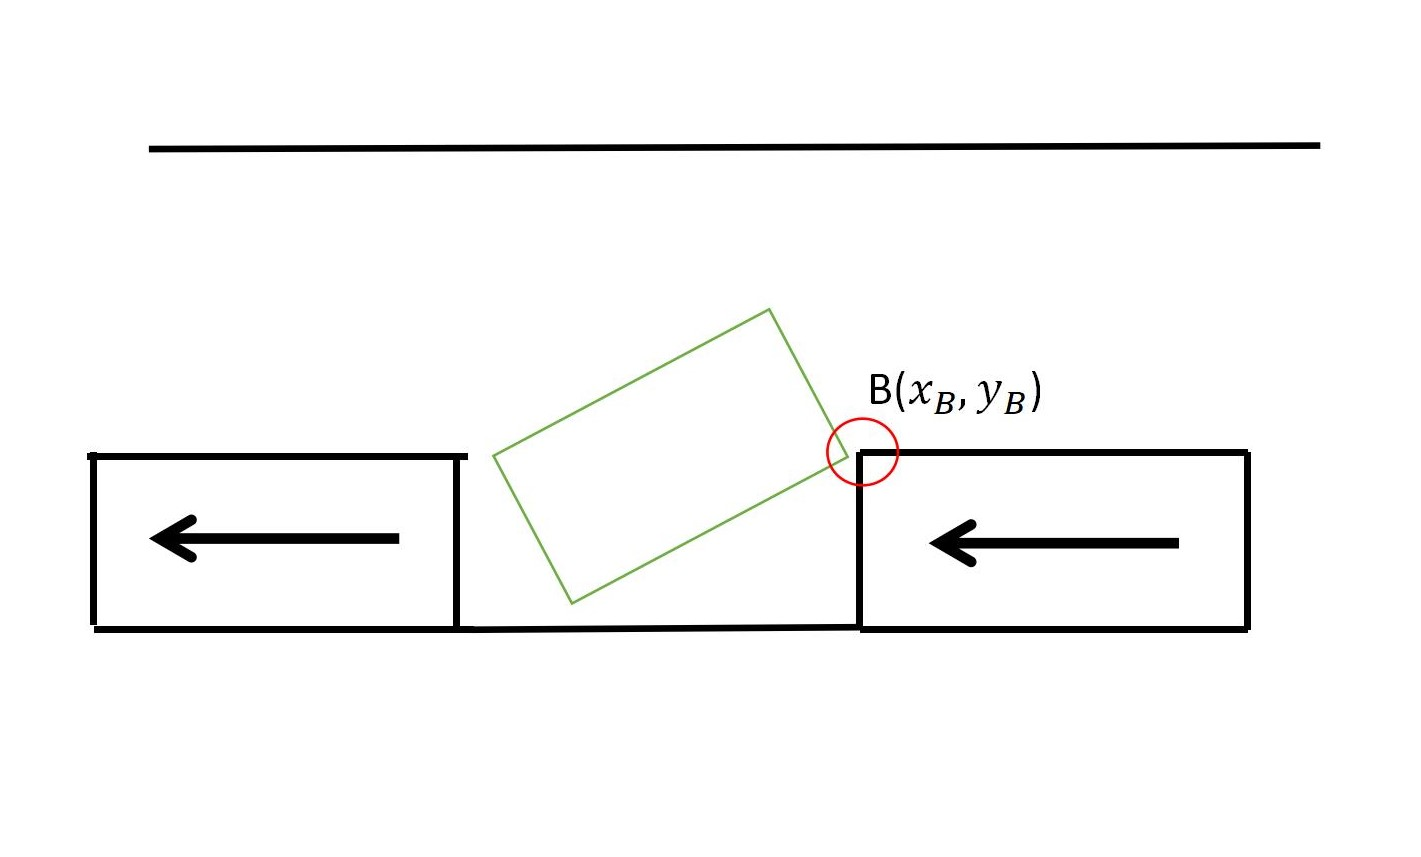
\includegraphics[width=1\textwidth]{13}
			% \subcaption{倾斜停车位}
			\label{fig:sample-figure-c}
		\end{minipage}
		\begin{minipage}[c]{0.3\textwidth}
			\centering
			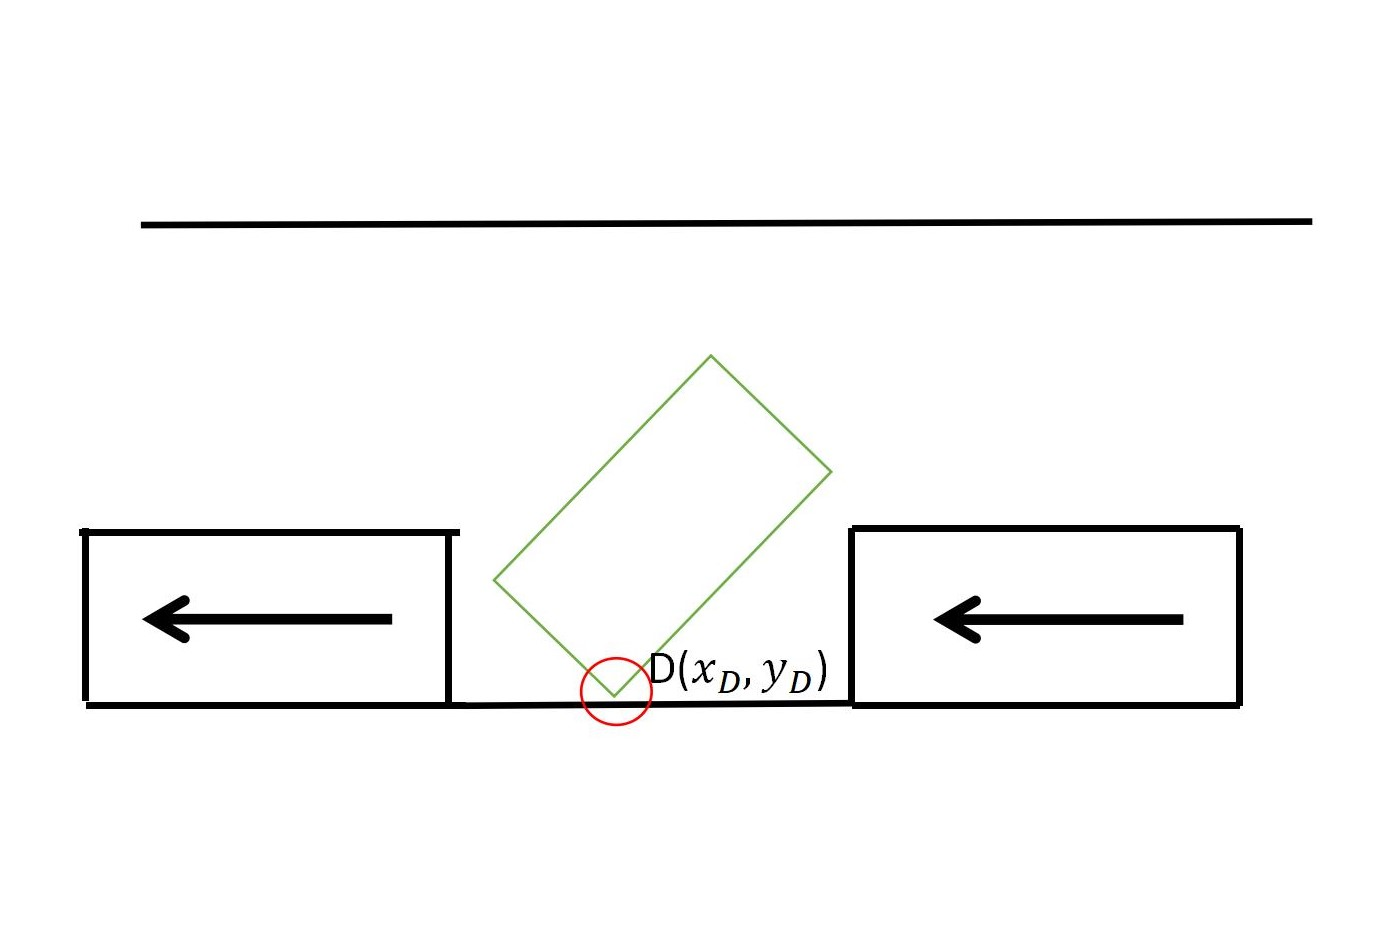
\includegraphics[width=1\textwidth]{14}
			% \subcaption{倾斜停车位}
			\label{fig:sample-figure-c}
		\end{minipage}
		\caption{平行泊车三种碰撞示意图}
		\label{fig:sample-figure}
	\end{figure}

	综合考虑碰撞约束、转向性能约束和几何关系约束,本文将以终点位置与车库边界的横向偏差、描述轨迹平缓程度的转角$\delta_0$和泊车时间$t$的加权和作为目标函数:
	\begin{equation}
		minJ(\delta_0,t_1,t_2)==\sqrt{{(y_{P6}-W_P)}^2+{(y_{P6}-W_P-W_R-\varepsilon)}^2}+K_1\delta_0+K_2(t_{1+}t_2+4\frac{\delta_0}{\delta_{0max}})
	\end{equation}
	\begin{equation}
		s.t.\left\{\begin{matrix}
			 y_A=y_P+\left(L+L_r\right)sin\theta+\frac{W_a}{2}cos\theta<W_R+W_P-\varepsilon
			\\ y_B=y_P+\left(L+L_r\right)sin\theta+\frac{W_a}{2}cos\theta>W_P
			\\x_B=H_P
			\\y_D=y_P-L_rsin\theta-\frac{W_a}{2}cos\theta>\varepsilon
			\\\delta_0\le\delta_{0max}	
		\end{matrix}\right.
	\end{equation}
	综上所述,只要确定前轮等效转角$\delta_0$、P2至P3段所对应的时间$t_1$和P4至P5段所对应的时间$t_2$这三个未知量,即可确定出前轮等效转角和时间之间的关系,根据式(8)、逆泊车轨迹起点P1以及转角与时间的曲线可以逐步递推出逆泊车轨迹上所有的位置点,即可得到$P1$->$P2$->$P3$->$P4$->$P5$->$P6$的运动轨迹。

	\item 10号垂直停车位轨迹规划
	
	垂直泊车轨迹规划分为辅助倒车轨迹和入库轨迹,仍采取逆泊车的思想,下面假设辅助倒车轨迹不会出现碰撞,重点考虑垂直入库P6至P1段。垂直泊车轨迹规划见图11。

	\begin{figure}[H]
		\centering
		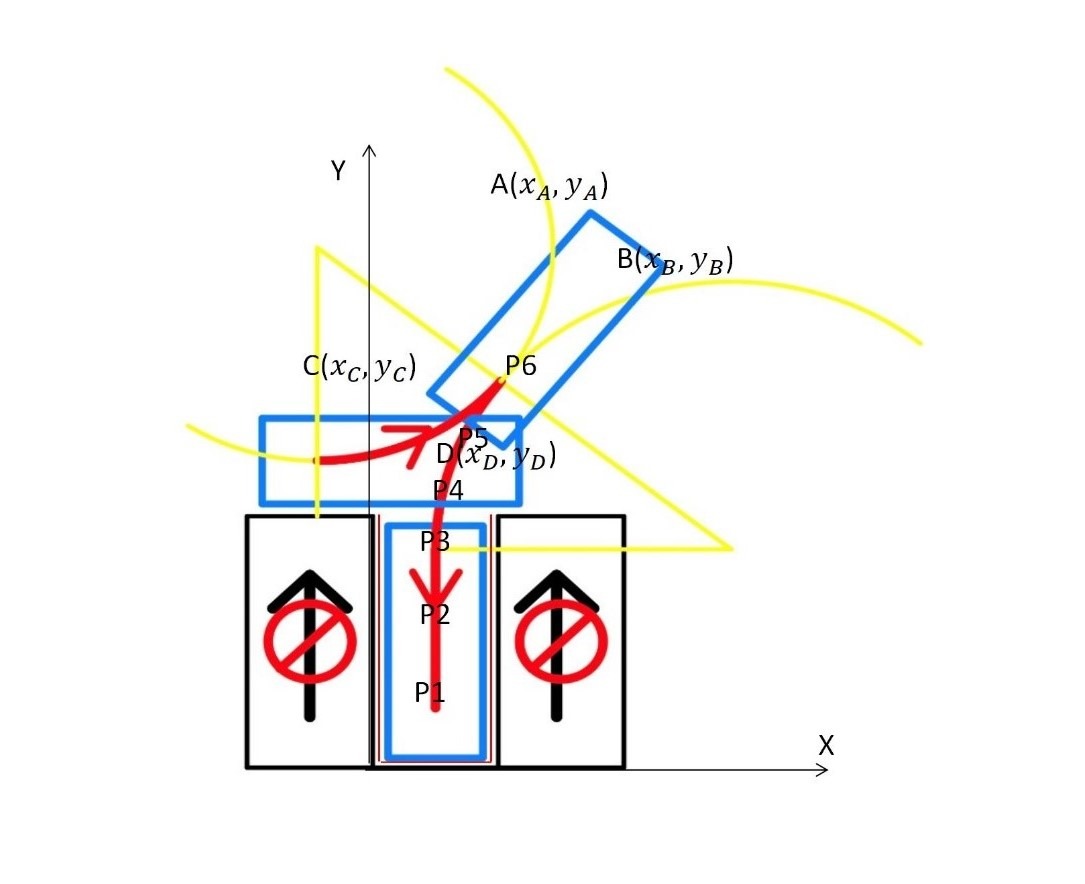
\includegraphics[width=.6\textwidth]{15}
		\caption{垂直泊车轨迹规划过程分析}
		\label{fig:circuit-diagram}
	\end{figure}


	在无人车垂直自动泊车过程中,要确保安全泊车,即无人车不能与其发生冲突或碰撞,因此需要满足的避碰条件和转向性能约束有:

	\begin{enumerate}
		\item 碰撞约束:
		\begin{itemize}
			\item 车辆外边缘左前顶点$A(x_A,y_A)$应避免与道路边界碰撞;
			\item 	车辆外边缘右后顶点$D(x_D,y_D)$应避免与泊车位左边界上顶点发生碰撞;
		\end{itemize}
		\item 转向性能约束:前轮转向角应不超过车辆最大转角值;
		\item 几何关系约束:车辆行驶过车中任意一点左边可由后轴中心坐标和车辆车身方位角通过几何表示;
		\begin{figure}[H]
			\centering
			\begin{minipage}[c]{0.3\textwidth}
				\centering
				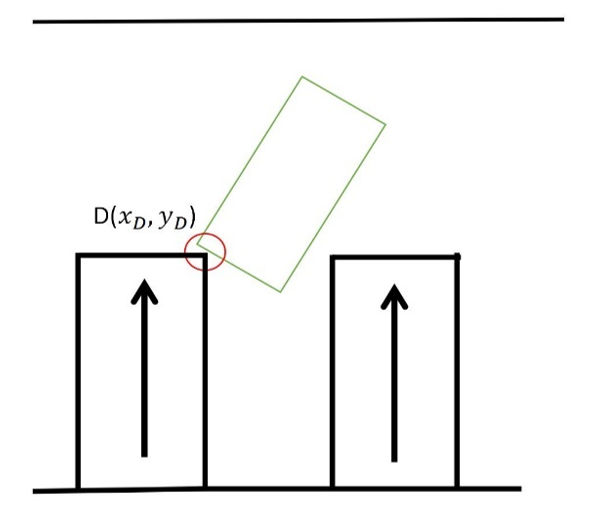
\includegraphics[width=1\textwidth]{16}
				% \subcaption{平行停车位}
				\label{fig:sample-figure-a}
			\end{minipage}
			\begin{minipage}[c]{0.3\textwidth}
				\centering
				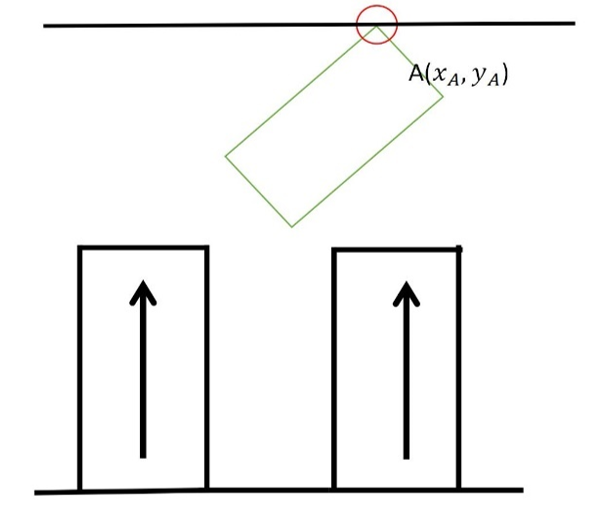
\includegraphics[width=1\textwidth]{17}
				% \subcaption{倾斜停车位}
				\label{fig:sample-figure-c}
			\end{minipage}
			\caption{垂直泊车两种碰撞示意图}
			\label{fig:sample-figure}
		\end{figure}
	
	\end{enumerate}
	综合考虑碰撞约束、转向性能约束和几何关系约束,本文将以终点位置与车库边界的横向偏差、描述轨迹平缓程度的转角$\delta_0$和泊车时间t的加权和作为目标函数:
	
	\begin{equation}
		minJ(\delta_0,t_1,t_2)==\sqrt{{(y_{P6}-W_P)}^2+{(y_{P6}-W_P-W_R-\varepsilon)}^2}+K_1\delta_0+K_2(t_{1+}t_2+4\frac{\delta_0}{\delta_{0max}})		
	\end{equation}
	\begin{equation}
		s.t. \left\{\begin{matrix}
			y_A=y_P+\left(L+L_r\right)sin\theta+\frac{W_a}{2}cos\theta<W_R+W_P-\varepsilon
			\\y_D=y_P-L_rsin\theta-\frac{W_a}{2}cos\theta>\varepsilon
			\\\delta_0\le\delta_{0max}	
		\end{matrix}\right.
	\end{equation}
		
	\item 31号倾斜停车位轨迹规划

	对于倾斜停车位的泊车轨迹的分析,与平行泊车位和垂直泊车位有所不同。我们将整个泊车过程分解为三段圆弧,并且由于倾斜泊车的特点,在泊车过程中的三段圆弧角度固定。因此,在对倾斜泊车轨迹进行规划时,目标函数不再是$\delta_0,t_1,t_2$,而是汽车距离墙体应尽可能远,即$y_p$尽可能小。
	
	\begin{figure}[H]
		\centering
		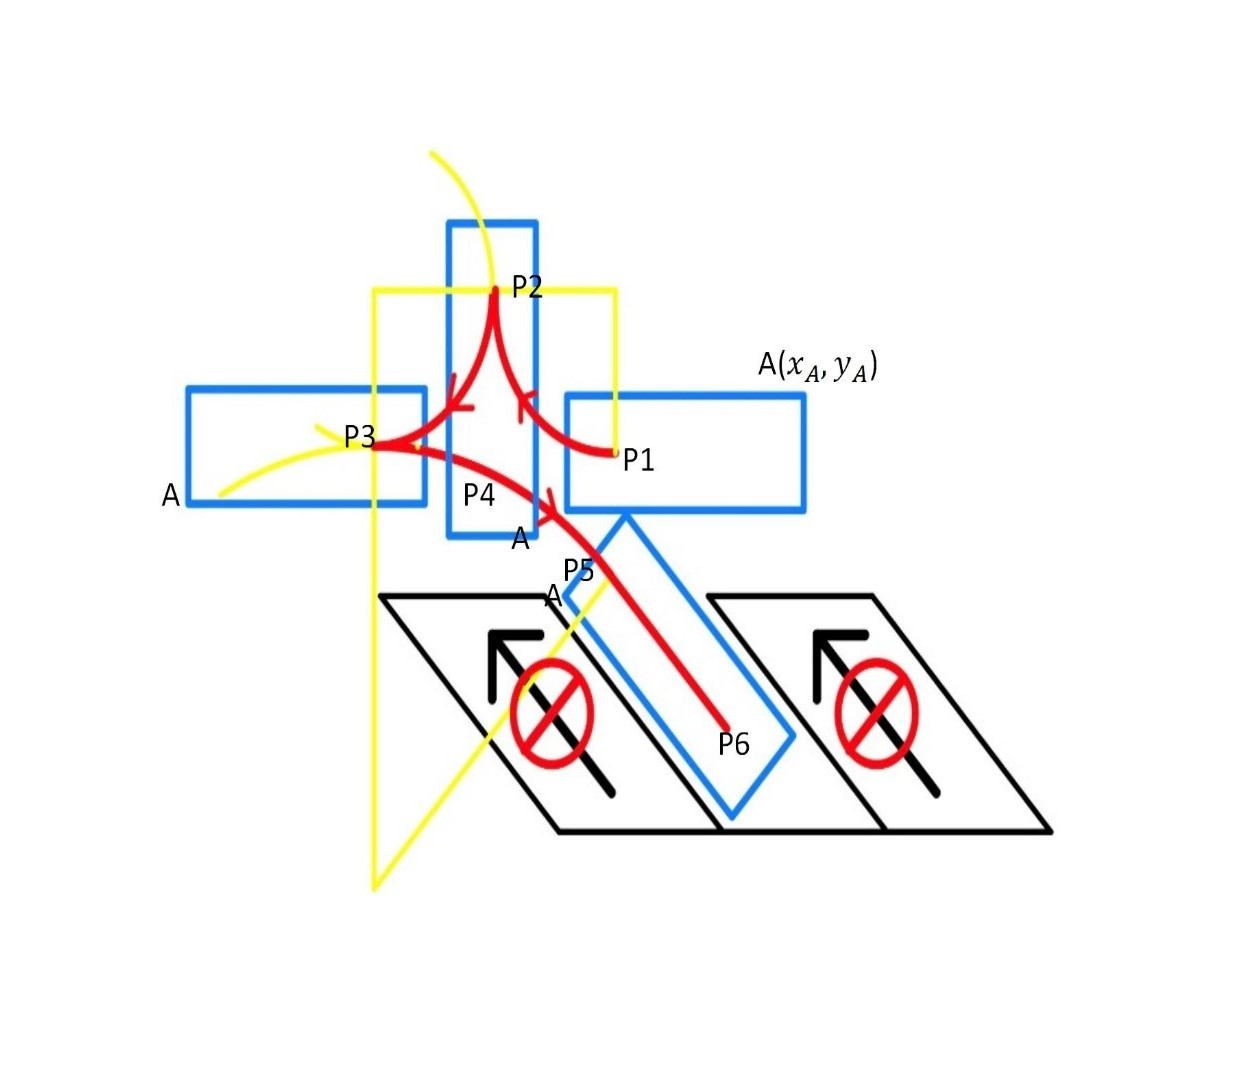
\includegraphics[width=.6\textwidth]{18}
		\caption{倾斜泊车轨迹规划过程分析}
		\label{fig:circuit-diagram}
	\end{figure}
	基于此,我们得出倾斜泊车轨迹的目标函数和约束条件为:
	\begin{equation}	
minJ(\delta_0,y_P6)==\sqrt{{(y_{P6}-W_{PX})}^2+{(y_{P6}-W_{PX}-W_{RX}-\varepsilon)}^2}+K_1\delta_0+K_2(t_{1+}t_2+4\frac{\delta_0}{\delta_{0max}})
	\end{equation}
	\begin{equation}
s.t.\left\{\begin{matrix}
	 y_B=y_P+\left(L+L_r\right)sin\theta+\frac{W_a}{2}cos\theta<{\sqrt{2(}W}_{RX}+W_{PX})-L_{PX}-\varepsilon
	\\ y_C=y_P-L_rsin\theta-\frac{W_a}{2}cos\theta>\varepsilon
	\\\delta_0\le\delta_{0max}	
\end{matrix}\right.
	\end{equation}
\end{enumerate}

\end{enumerate}
	\subsubsection{模型的求解}
	在上文的逆泊车轨迹规划基础上,只要$\delta_0,t_1,t_2$三个未知参数的不同取值进行组合,可以得到不同的轨迹曲线,进而可以得到不同的泊车路径。当三个未知参数选取合适的取值范围,可以取到所有可行的泊车轨迹。本文将转向角$\delta_0$取值范围设定在$0$~$0.6rad$,将$t_1$,$t_2$取值范围设定在$0~5s$,以$0.05rad$角度间隔和$0.5s$的时间间隔取遍所有的$\delta_0$和$t_1$,$t_2$取值范围,即可以得到所有满足可行泊车轨迹簇。下文将运用粒子群算法求得满足约束条件的一条最优最优轨迹。
	\begin{enumerate}
		\item 粒子群算法
		
		粒子群优化算法(Particle swarm optimization,简称PSO)是一种进化计算技术。源于对鸟群捕食的行为研究。粒子群优化算法的基本思想:是通过群体中个体之间的协作和信息共享来寻找最优解。

		PSO算法就是模拟一群鸟寻找食物的过程,每个鸟就是PSO中的粒子,也就是我们需要求解问题的可能解,这些鸟在寻找食物的过程中,不停改变自己在空中飞行的位置与速度。粒子仅具有两个属性:速度和位置,速度代表移动的快慢,位置代表移动的方向。每个粒子在搜索空间中单独的搜寻最优解,并将其记为当前个体极值,并将个体极值与整个粒子群里的其他粒子共享,找到最优的那个个体极值作为整个粒子群的当前全局最优解,粒子群中的所有粒子根据自己找到的当前个体极值和整个粒子群共享的当前全局最优解来调整自己的速度和位置。

			  \begin{figure}[H]
				\centering
				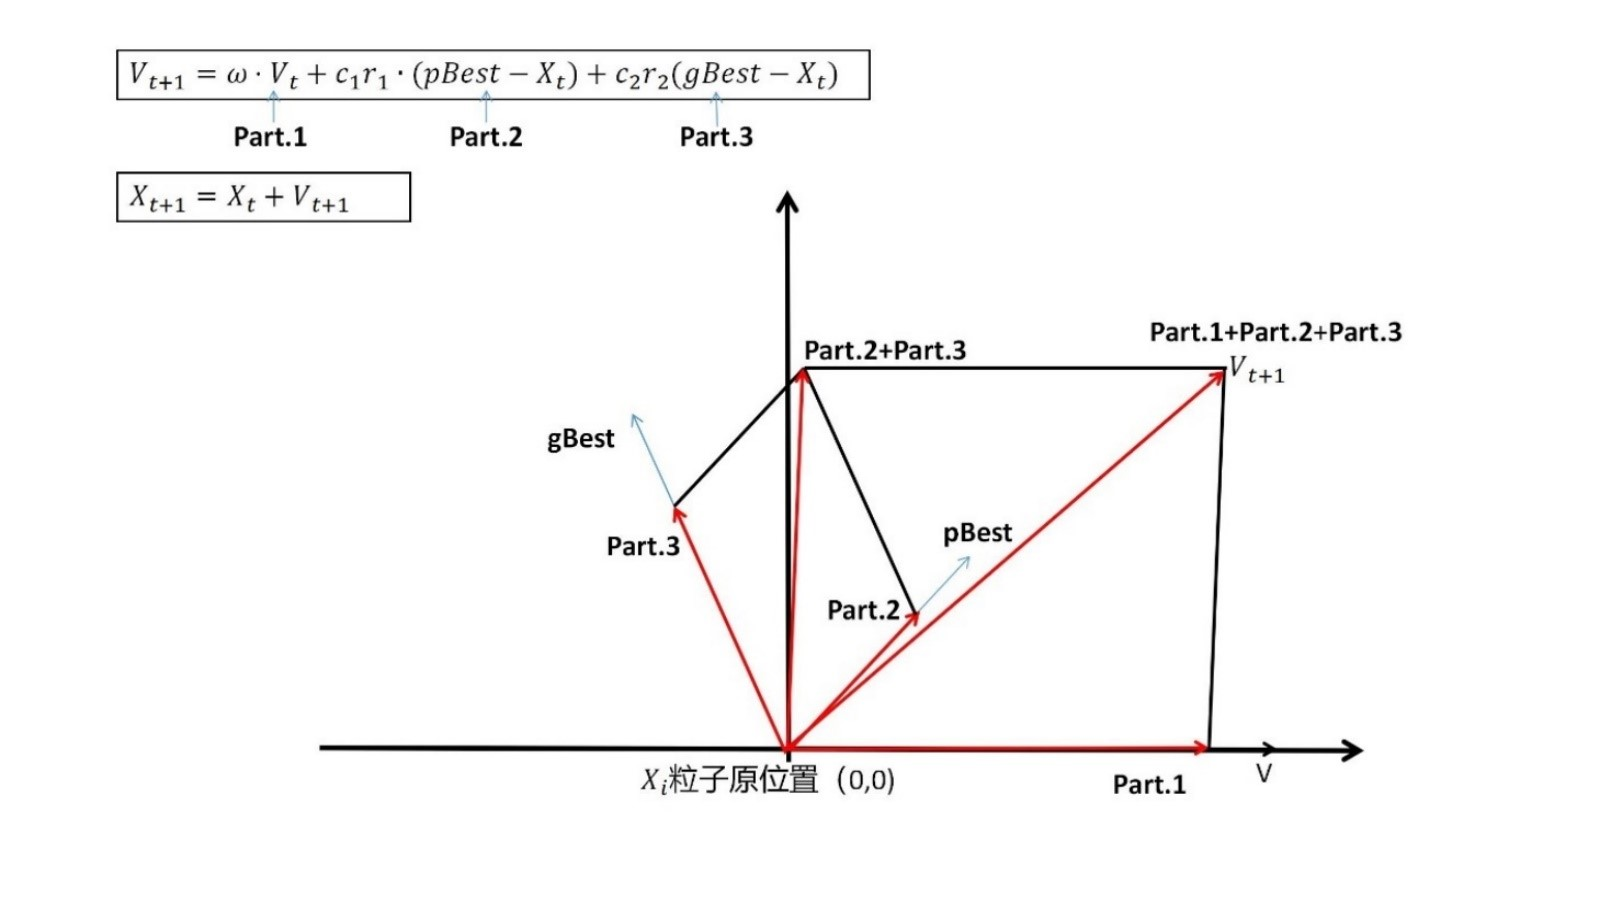
\includegraphics[width=0.7\textwidth]{粒子群}
				\caption{粒子群算法示意图}
				\label{fig:circuit-diagram}
			\end{figure}

		PSO初始化为一群随机粒子(随机解)。然后通过迭代找到最优解。在每一次的迭代中,粒子通过跟踪两个“极值”$(pbest,gbest)$来更新自己。在找到这两个最优值后,粒子通过以下两个的公式来更新自己的速度和位置。
		
		\begin{equation}
			V_{t+1}=\omega\cdot V_t+c_1r_1\cdot(pBest-X_t)+c_2r_2\cdot(gBest-X_t)
		\end{equation}
		\begin{equation}
			x_{t+1}=x_t+v_{t+1}
		\end{equation}

		式中$\omega$为速度的惯性权重,其值较大是代表例子全局寻优能力强,局部寻优能力弱;值较小时代表全局寻优能力弱,局部寻优能力强;$c_1$为粒子的个体学习因子;$c_2$为粒子的社会学习因子;$r_1$为[0,1]范围内的随机数。

		公式(16)的第一部分$\omega\cdot V_t$称为记忆项,表示维持上次速度大小和方向的趋势,反应例子的运动习惯;公式(16)的第二部分$c_1r_1\cdot(pBest-X_t)$称为自身认知项,是从当前点指向粒子自身最好点的一个矢量,表示粒子的动作来源于自己经验的部分,有向历史最佳位置运动的趋势;公式(16)的第三部分$c_2r_2\cdot(gBest-X_t)$称为群体认知项,是一个从当前点指向种群最好点的矢量,反映了粒子间的协同合作和知识共享。粒子将自己的经验和同伴中最好的经验结合决定下一步的运动。以上面式(16)和式(17)公式为基础,形成了PSO的标准形式。其算法示意图如下,
		\item 算法设计与求解
		
		根据粒子群算法原理,我们设计出相应的轨迹优化算法伪代码如下:
		
		\begin{algorithm}
			% \begin{small}
			  \caption{粒子群优化轨迹算法}
			\KwOut{$\delta_0$,$t_1$,$t_2$}
			初始化粒子群,设置粒子群个数N
			\While{最大迭代次数为达到活最小误差未达到}{
			
			\For {每个粒子}
			{计算其适应度
			  \If {适应度优于粒子历史最佳值}
			  {
				更新历史最佳个体

			  }}
				\If {当前最佳粒子优于群历史最佳粒子}{
				  用当前群最佳粒子更新$Best$
				}
				\For{每个粒子}
				{

				更新粒子速度;
				
				在满足轨迹约束条件的前提下,更新粒子位置;

				
				}
				}
			return $\delta_0$,$t_1$,$t_2$;
			% \end{small}
		\end{algorithm}
		  
		完整代码展示于附录2。最终结果展示如下:
		  \begin{enumerate}
			  \item 泊车轨迹
			  
			%   \begin{figure}[H]
			% 	\centering
			% 	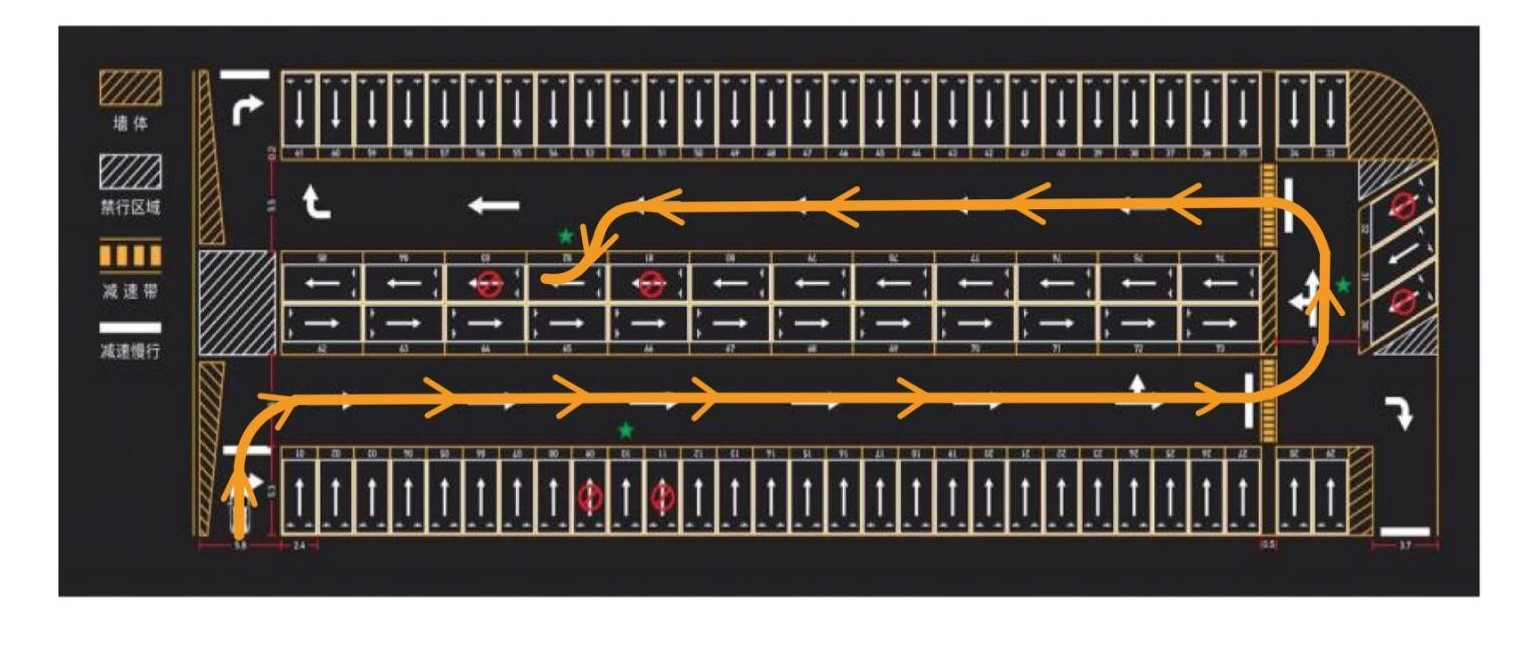
\includegraphics[width=1\textwidth]{22}
			% 	\caption{}
			% 	\label{fig:circuit-diagram}
			% \end{figure}

			\begin{figure}[H]
				\centering
				\begin{minipage}[c]{0.4\textwidth}
					\centering
					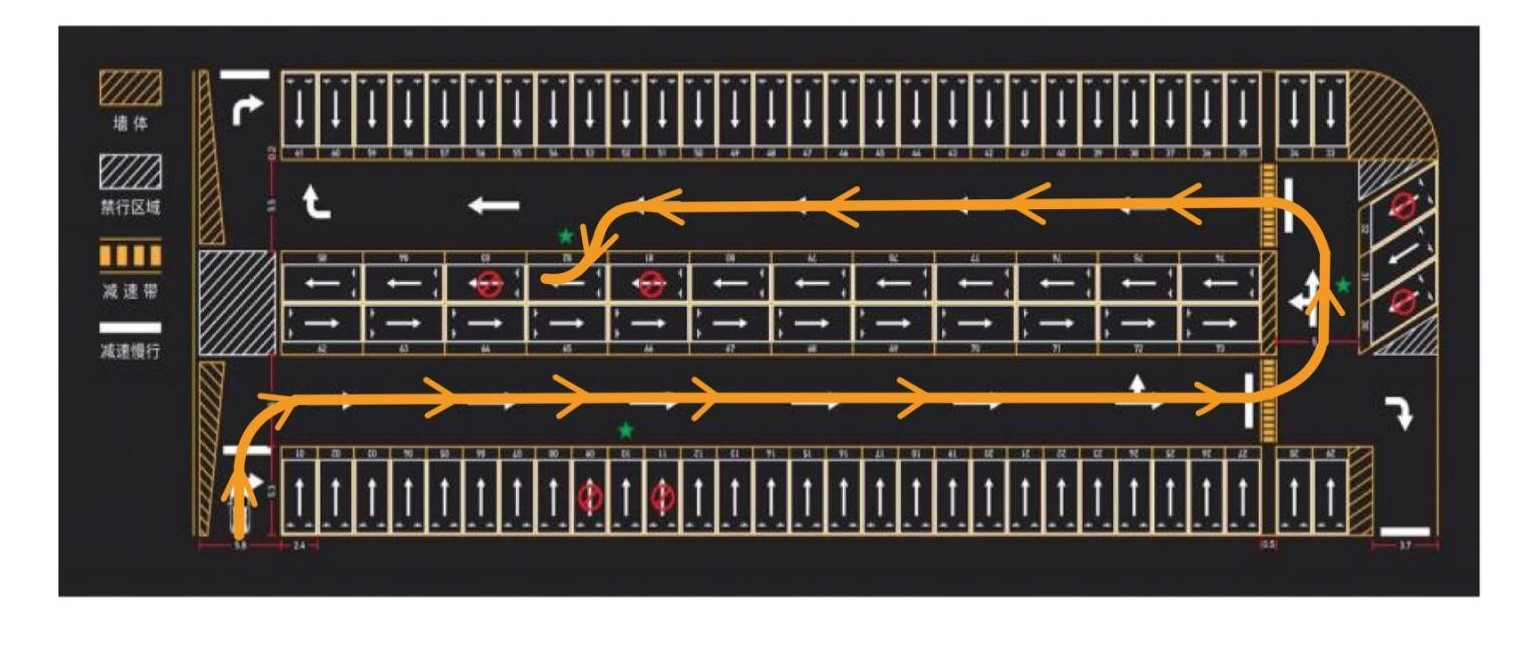
\includegraphics[width=0.95\textwidth]{22}
					% \subcaption{平行停车位}
					\label{fig:sample-figure-a}
				\end{minipage}
				\begin{minipage}[c]{0.4\textwidth}
					\centering
					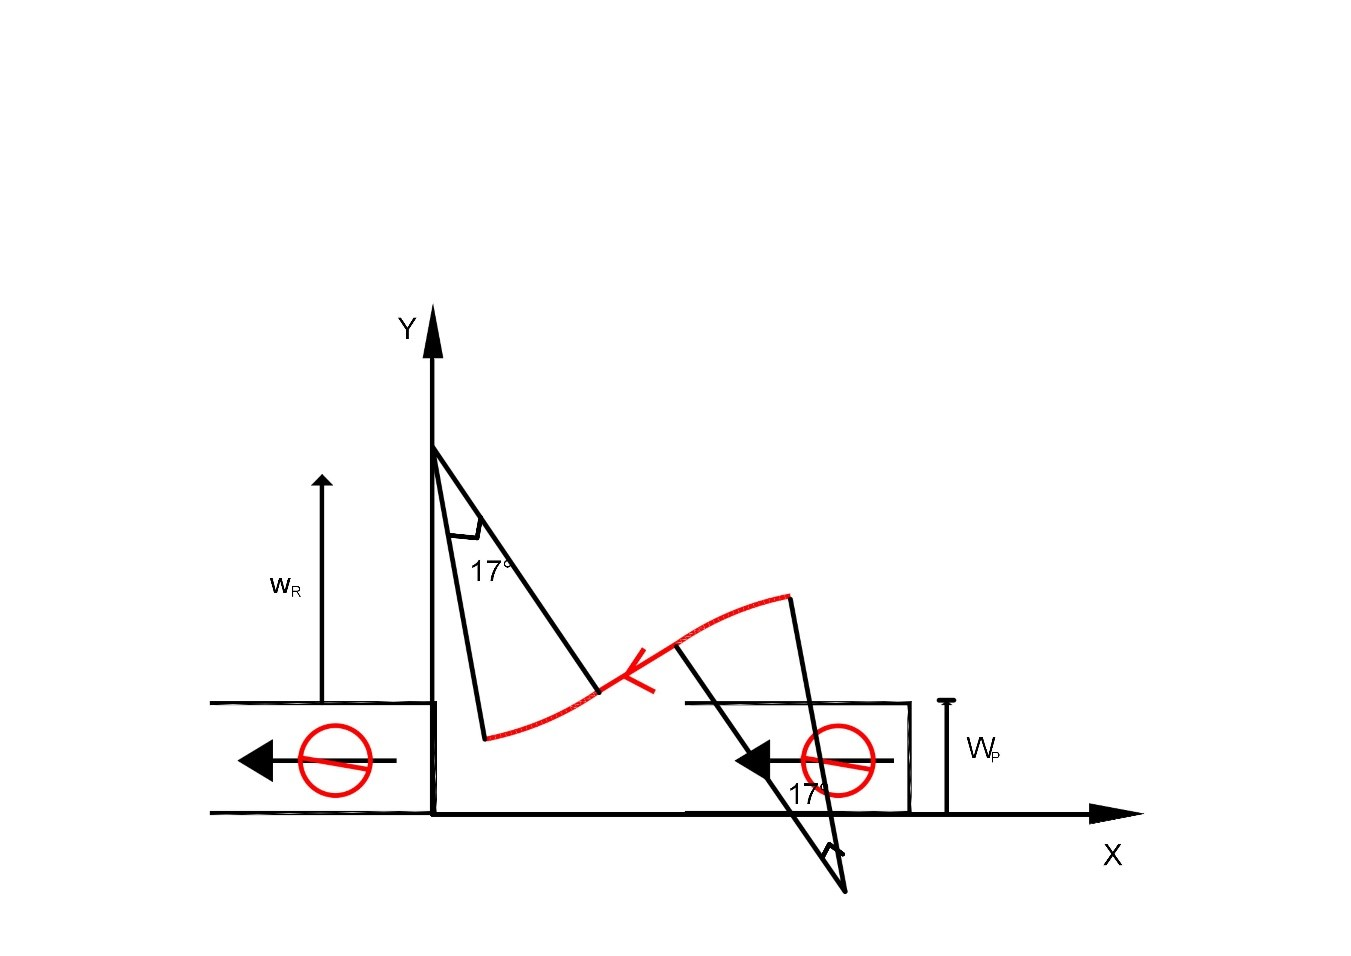
\includegraphics[width=0.95\textwidth]{111}
					% \subcaption{倾斜停车位}
					\label{fig:sample-figure-c}
				\end{minipage}
				\caption{从初始位置到82号平行停车位的泊车轨迹}
				\label{fig:sample-figure}
			\end{figure}

			% \begin{figure}[H]
			% 	\centering
			% 	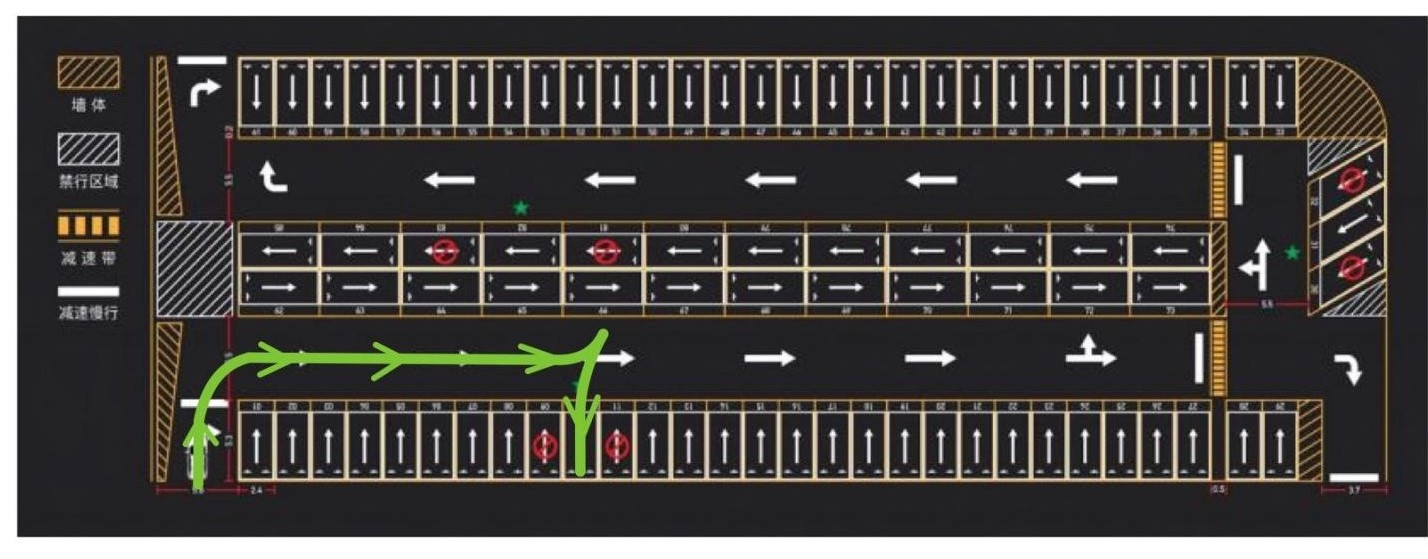
\includegraphics[width=1\textwidth]{23}
			% 	\caption{从初始位置到10号平行停车位的泊车轨迹}
			% 	\label{fig:circuit-diagram}
			% \end{figure}

			\begin{figure}[H]
				\centering
				\begin{minipage}[c]{0.4\textwidth}
					\centering
					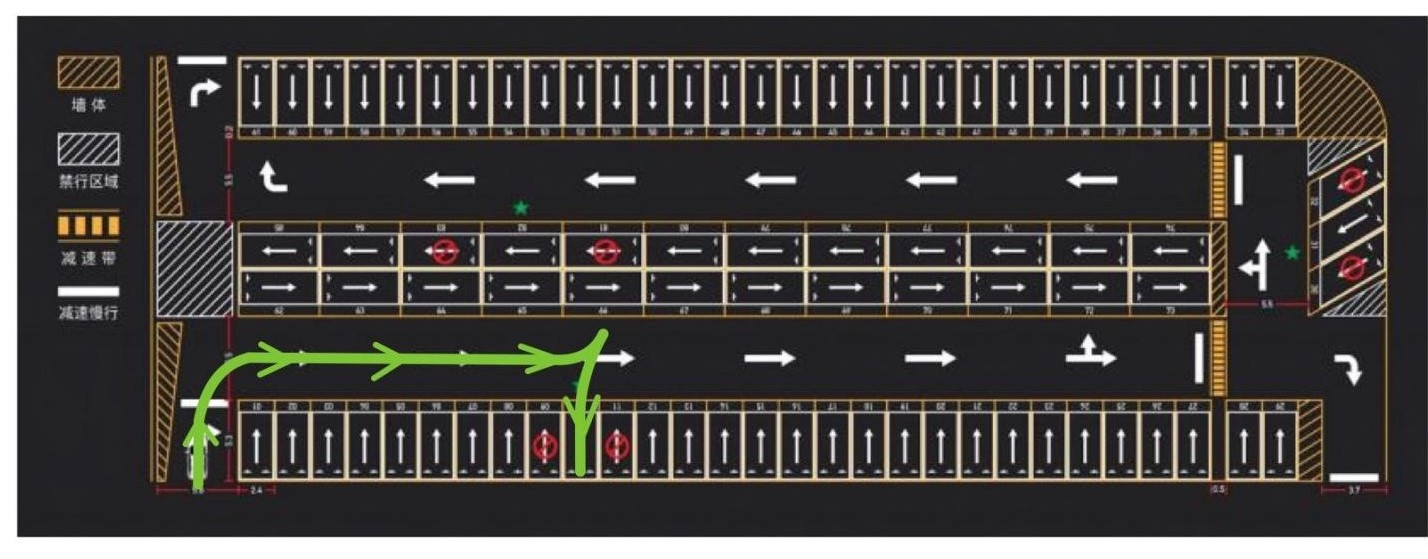
\includegraphics[width=0.95\textwidth]{23}
					% \subcaption{平行停车位}
					\label{fig:sample-figure-a}
				\end{minipage}
				\begin{minipage}[c]{0.4\textwidth}
					\centering
					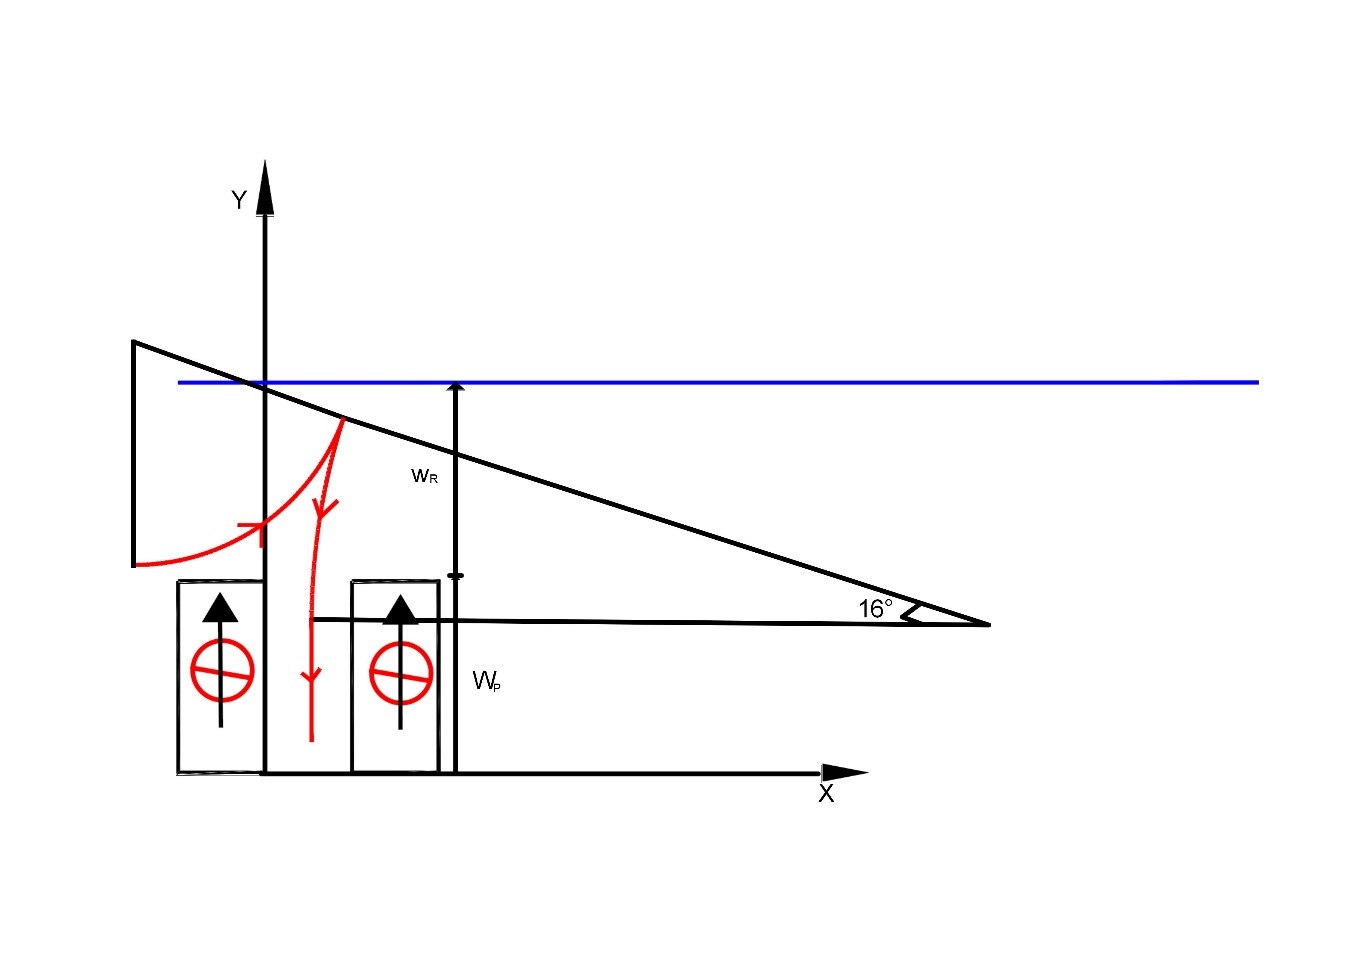
\includegraphics[width=0.95\textwidth]{222}
					% \subcaption{倾斜停车位}
					\label{fig:sample-figure-c}
				\end{minipage}
				\caption{从初始位置到10号平行停车位的泊车轨迹}
				\label{fig:sample-figure}
			\end{figure}


			% \begin{figure}[H]
			% 	\centering
			% 	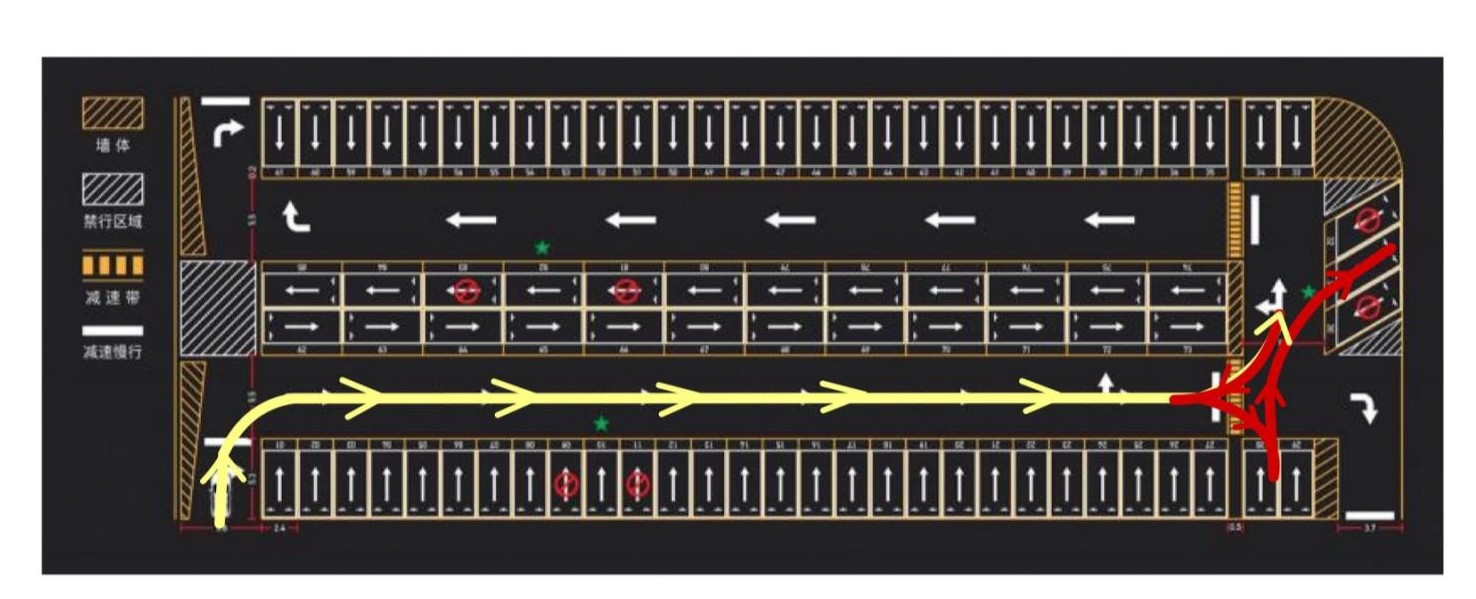
\includegraphics[width=1\textwidth]{24}
			% 	\caption{从初始位置到31号倾斜停车位的泊车轨迹}
			% 	\label{fig:circuit-diagram}
			% \end{figure}

			\begin{figure}[H]
				\centering
				\begin{minipage}[c]{0.4\textwidth}
					\centering
					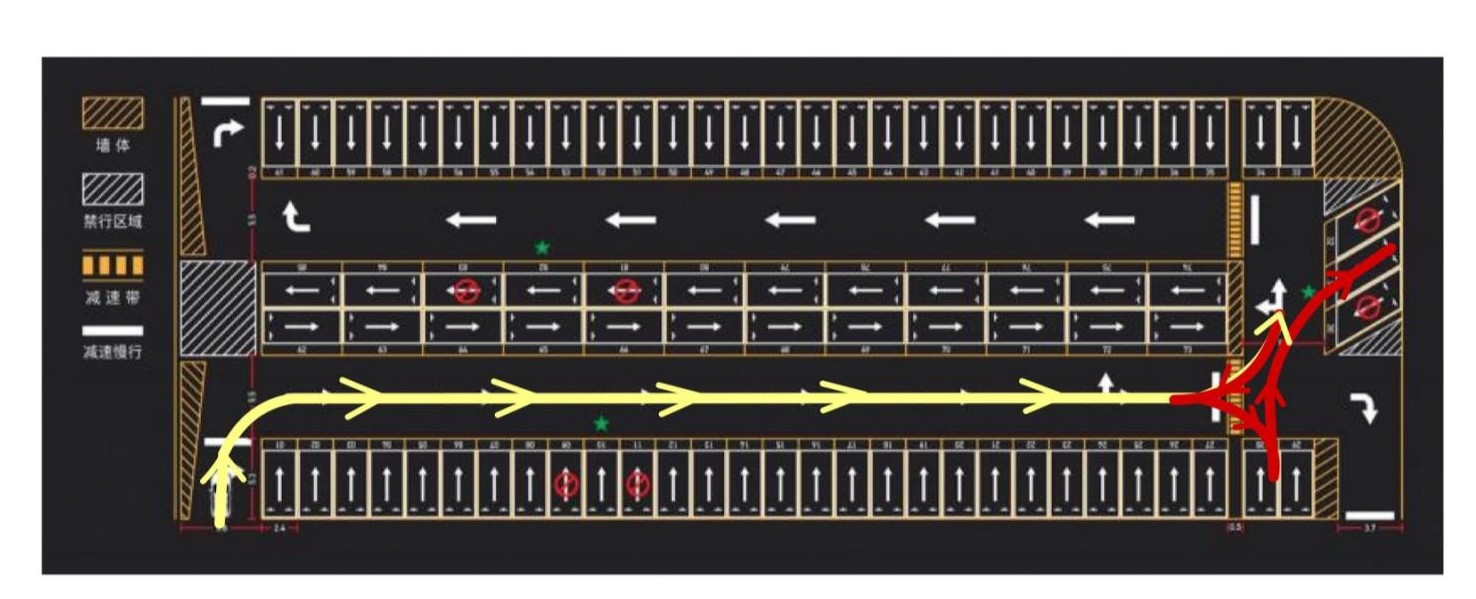
\includegraphics[width=0.95\textwidth]{24}
					% \subcaption{平行停车位}
					\label{fig:sample-figure-a}
				\end{minipage}
				\begin{minipage}[c]{0.4\textwidth}
					\centering
					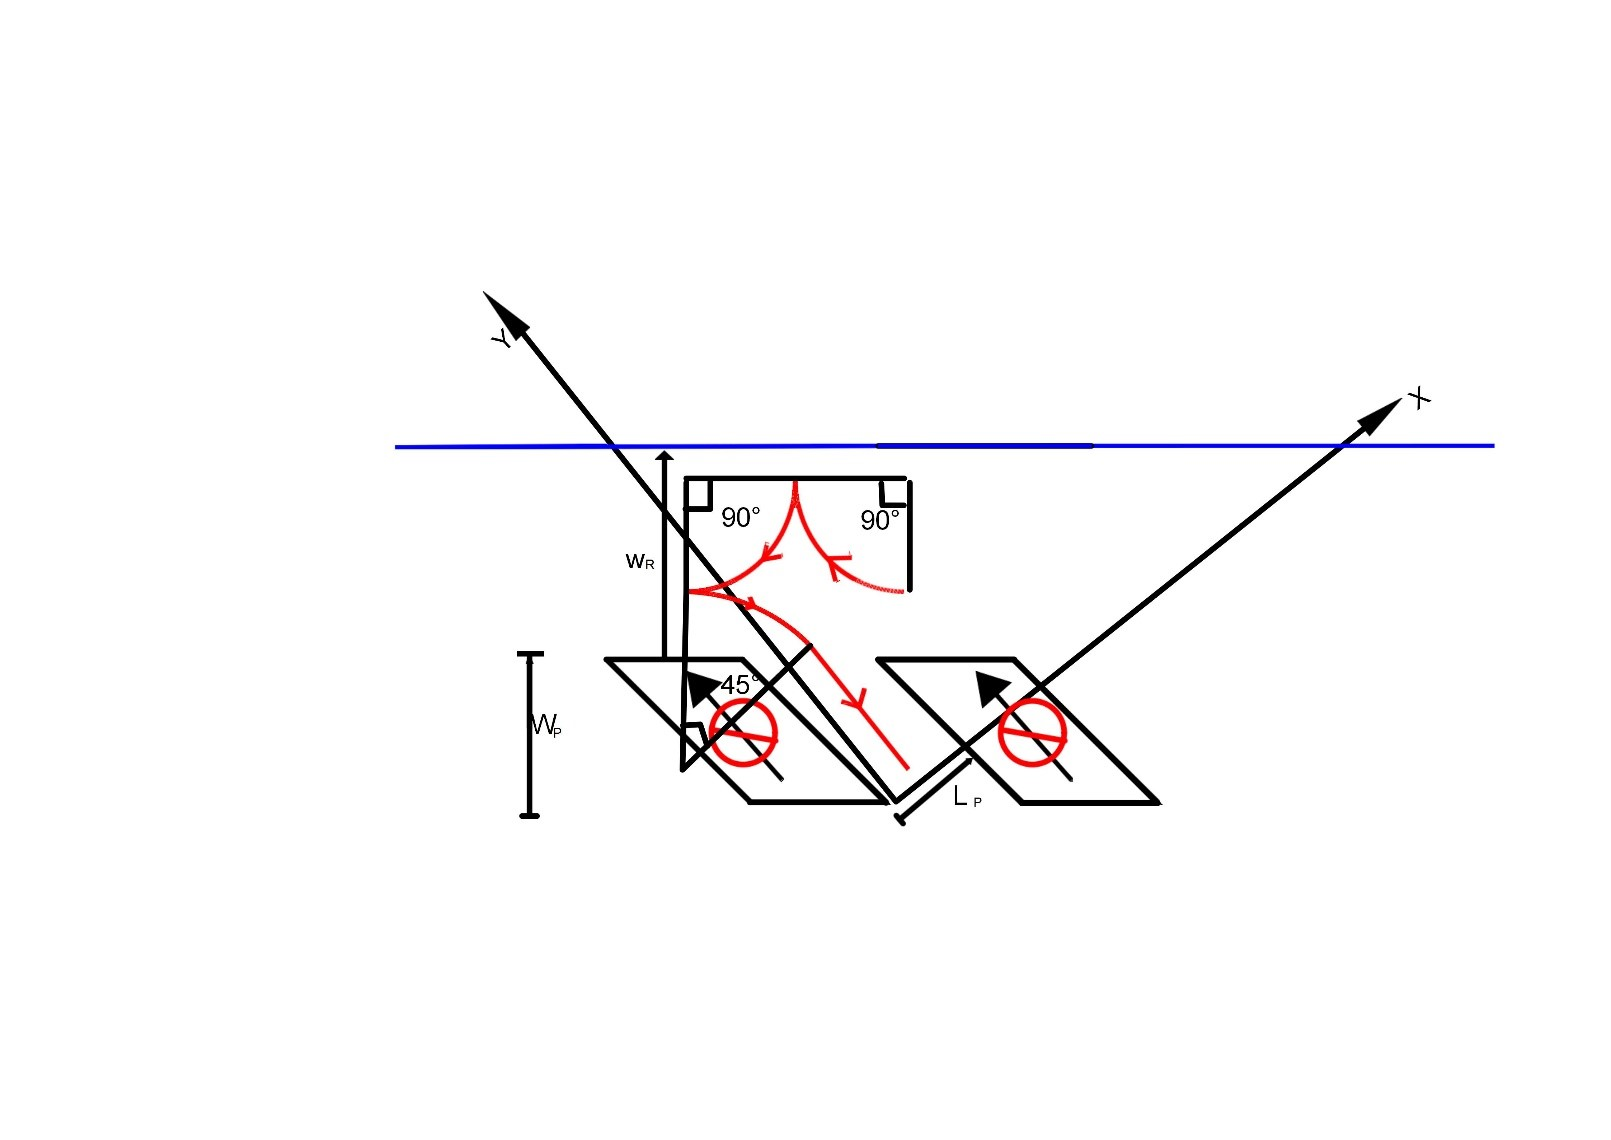
\includegraphics[width=0.95\textwidth]{333}
					% \subcaption{倾斜停车位}
					\label{fig:sample-figure-c}
				\end{minipage}
				\caption{从初始位置到31号倾斜停车位的泊车轨迹}
				\label{fig:sample-figure}
			\end{figure}

			  \item 角速度
			  \begin{figure}[H]
				\centering
				\begin{minipage}[c]{0.325\textwidth}
					\centering
					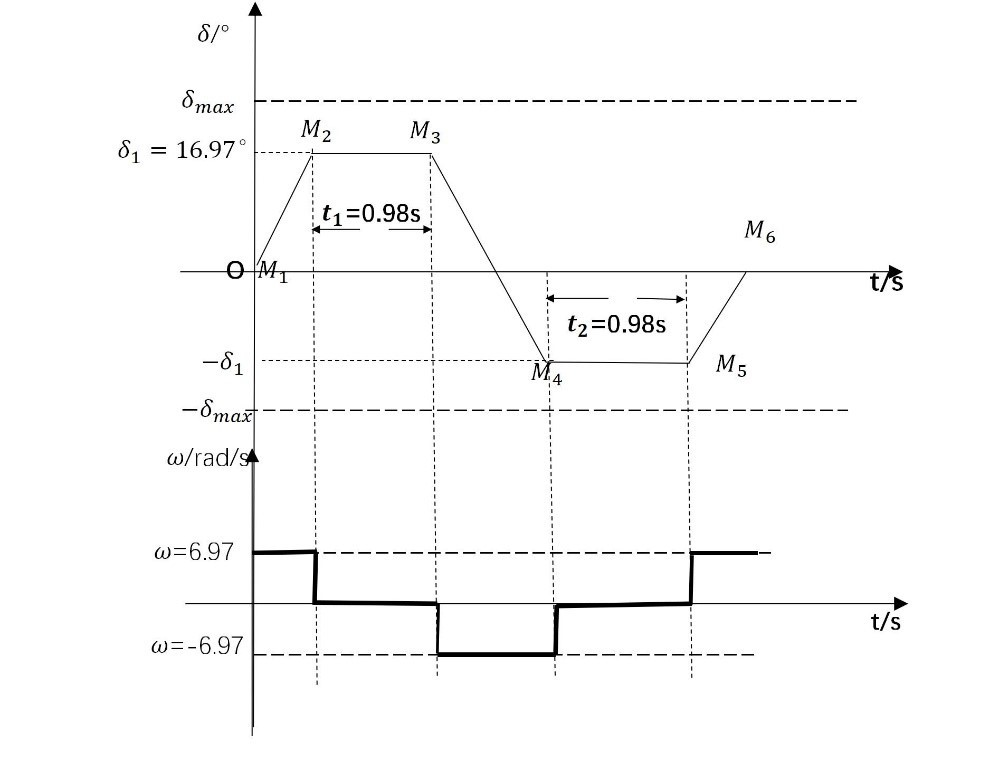
\includegraphics[width=0.9\textwidth]{25}
					\subcaption{从初始位置到82号平行停车位的角速度变化}
					\label{fig:sample-figure-a}
				\end{minipage}
				\begin{minipage}[c]{0.325\textwidth}
					\centering
					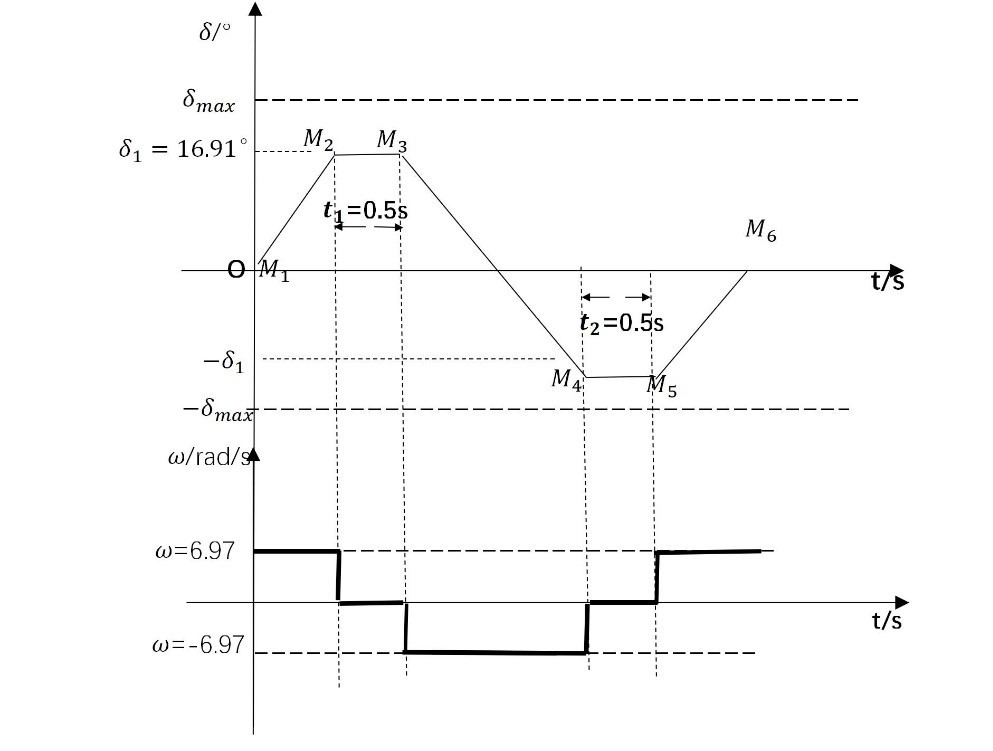
\includegraphics[width=0.9\textwidth]{26}
					\subcaption{从初始位置到10号垂直停车位的角速度变化}
					\label{fig:sample-figure-c}
				\end{minipage}
				\begin{minipage}[c]{0.325\textwidth}
					\centering
					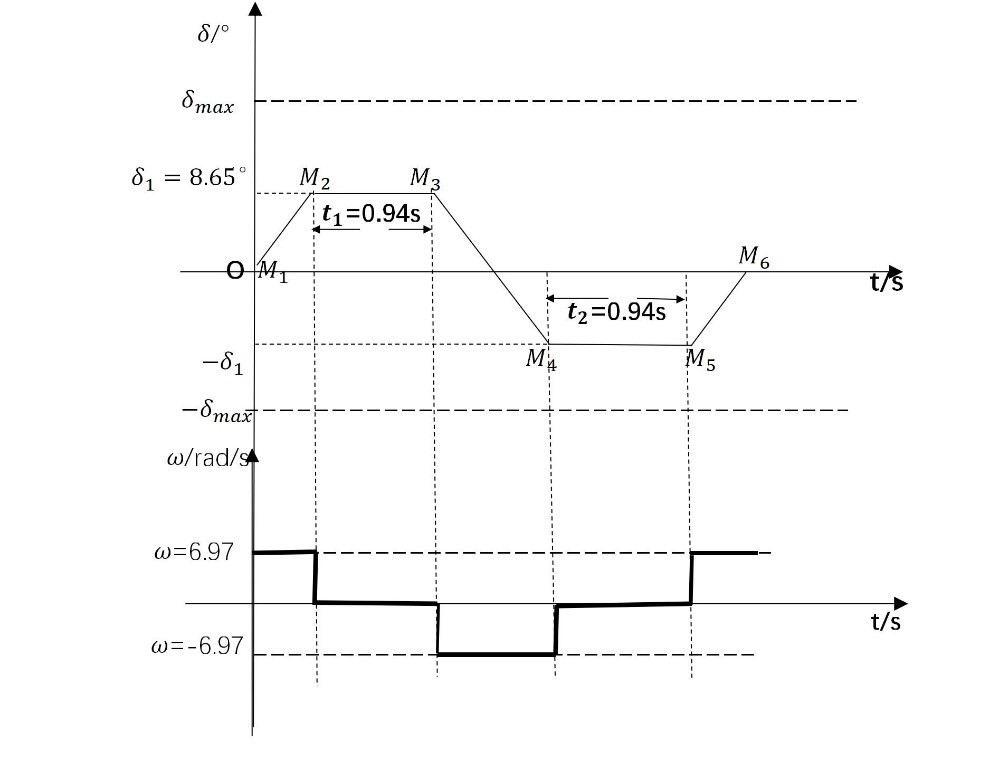
\includegraphics[width=0.9\textwidth]{27}
					\subcaption{从初始位置到31号倾斜停车位的角速度变化}
					\label{fig:sample-figure-c}
				\end{minipage}
				\caption{从初始位置到三种停车位的角速度变化}
				\label{fig:sample-figure}
			\end{figure}
		  \end{enumerate}

	\end{enumerate}
	



	\subsection{问题三模型的建立与求解}
	最优停车位的目标为安全情况下泊车过程最短时间,因此将整个停车时间分为四个时间段考虑,分别为直线加速路程时间、转弯时间、减速带减速时间和三种类型车位泊车时间,根据可用车位的具体位置考虑泊车总时间由哪些时间段组成,到达车位的时间和最小即此车位为最优车位。

	为了方便问题研究,本文将停车场路径分为三个区域段,因为车辆一旦进入停车场,只能前行寻找车位,不能够逆行寻找车位,通过确定可行车位在第几段区域内,即可确定该泊车过程中所需时间有哪些时间段组成。具体三个区域段见图18 :

	\begin{figure}[h]
		\centering
		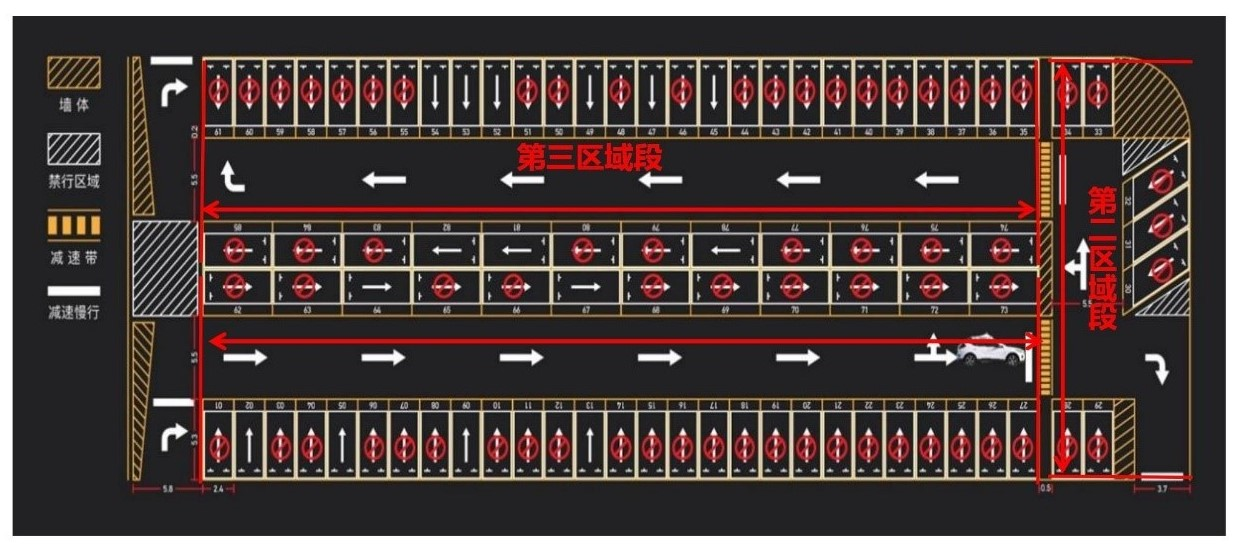
\includegraphics[width=.8\textwidth]{28}
		\caption{停车场区域划分图}
		\label{fig:circuit-diagram}
	\end{figure}


	由上图可见,在第一区域段为车库入口到第一个减速带;第二区域段为两个减速带之间的区域;第三段区域段为第二个减速带至车库上方出口。

	本题题目已给定车的初始位置,并且在寻找最优停车位时由于只能前行,不能倒退行驶寻找车位,因此只需要考虑第二、第三区域段的可用停车位。根据当前停车场停车位状态,第二阶段无可用停车位,因此只需考虑第三区域段的可用停车位。

	\subsubsection{模型的建立}
	以第二题三种最佳泊车轨迹为基础,由于汽车的初始位置位于减速带前后五米的范围内,因此我们可以假定汽车的初始速度为10km/h,也为倒车允许的最大速度,以及初始位置位于减速带前1.2m,因此可以分为以下四个阶段:
	\begin{enumerate}
		\item 减速带阶段
		
		减速带行驶所需时间:汽车经过减速带匀速驶入第二区域段所需的时间为
		\begin{equation}
			t_1=\frac{L_0}{v_1}
		\end{equation}
		式中:$L_0$为起始位置到减速带的距离。
		\item 转弯阶段
		
		车辆在第二阶段内行驶轨迹为两段四分之一的圆周,在这一区域段里直线运动很短,忽略不计,此过程继续保持基于初始速度,基于问题二的转弯模型,从而可以求得汽车在第二阶段的时间
		\begin{equation}
			t_2=\frac{2\pi R_{min}\times2}{{4v}_1}
		\end{equation}
		\item 直行阶段
		
		此直线运动可分为三段:第一段以油门最大加速度$a_1$作匀加速直线运动,加速至限制的最大速度$v_{max}$,此段时间记为$t_3$;第二阶段是以$v_{max}$匀速行驶,此段时间记为$t_4$;最后以油门最大减速度$a_2$作匀减速直线运动至速度为$v_1$,此段时间记为$t_5$。
		
		最终得到直行阶段的时间为
		\begin{equation}
			t_3+t_4+t_5=\frac{v_{max}-v_1}{a_1}+\frac{{S-S}_1-S_2}{v_{max}}+\frac{v_{max}-v_1}{a_2}
		\end{equation}
		式中:$S_1$为加速过程行驶距离;$S_2$为匀速行驶距离;$S_3$为减速过程的行驶距离。
		\item 泊车阶段
		
		问题二中已找出最佳的泊车路径,此时泊车的时间即是最短时间,记为$t_6$。
		

	\end{enumerate}
	\subsubsection{模型的求解}
	为求解此问题,我们设计的算法步骤如下:
	\begin{enumerate}
		\item [$step1$]设置停车位类,其属性包括车位至入口的距离$x$、车库类型$properties$、车位是否被占用$isOccupy$(0表示未被占用、1表示已被占用)、车库所在位置$position$(0表示第一段区域、1表示第二段区域、2表示第三段区域);
		
		设置汽车类,其属性包括汽车至入口的距离$x$。
		\item [$step2$]初始化85个停车位类和一个汽车类。根据题意要求,2、5、9、13、45、52、53、54、64、67、78、81、82号停车位的初始化$isOccupy$值设置为0,其余均位1。
		\item [$step3$]计算汽车到每个$isOccupy$值为0的车库的时间。(停车花费时间的计算规则为:减速带阶段时间+转弯阶段时间+直行阶段时间+泊车阶段时间)
		\item [$step4$]找出停车花费时间最少的车位,即为所求的最优停车位。
	\end{enumerate}
	
	算法中使用了嵌套双循环,故时间复杂度为$O(n^2)$。

	最终求得最优停车位为78号停车位,停车花费的时间$t_{min}$约为11s,泊车轨迹如下图所示。
	\begin{figure}[h]
		\centering
		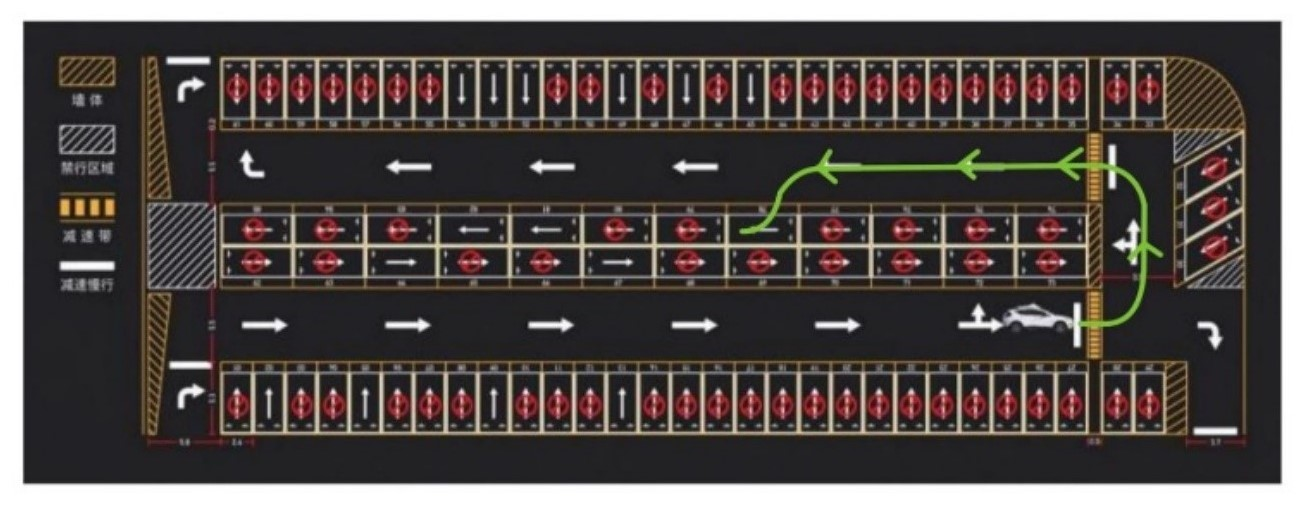
\includegraphics[width=.9\textwidth]{29}
		\caption{从当前位置到78号平行泊车停车位的泊车轨迹}
		\label{fig:circuit-diagram}
	\end{figure}






	\subsection{问题四模型的建立与求解}
	\subsubsection{模型的建立}
	针对于此问题,题目要求我们以第三问所给的车辆初始位置,将此车辆命名为A车辆,假设在当前状态下每小时内从入口进入和从出口离开停车场的车辆均为 30 辆,在此过程中会导致车辆的进入和离开,进一步导致停车位会被随机占用或释放。与问题三不同是停车场变为了一个动态过程,由于每小时进入和离开的车辆均为30辆,因此在本题中我们假定两分钟有一辆车的驶入与离开。以当前车辆为研究对象,停车场的动态过程对研究对象的影响主要体现在以下两个方面:
	\begin{enumerate}
		\item 在两分钟内,当前车辆前方由于有车辆离开,停车位由原来的被占用变为释放,进而会导致A车辆的最优目标停车位改变。
		\item 在两分钟内,有新的车辆驶入车库,并且驾驶速度大于A车辆的车速(车辆的宽度为1.8m,道路的宽度为5.5m,可满足后方车辆对A车辆进行超车的条件),因此可以进行超车,进而导致A车辆的前面的最优目标停车位由原来的释放状态变为占用状态,使得A车辆需要重新寻找最优目标车位。
	\end{enumerate}

	基于问题三的模型与算法,只需要对其算法进行补充,即可进行求解
	
	\subsubsection{模型的求解}
	针对问题四,我们增加车辆随机进出的算法模块(展示于附录3)。使用随机数设置车辆离开和进入的车位,每次车位状态发生变化时,重新规划最优停车位。
	
	算法给出最优车停车位,便可确定该停车位的类型和位置,便可设计出从当前位置到最优停车位的行驶轨迹的仿真结果。

\section{模型的评价、改进与推广}
\subsection{模型的评价}
\begin{enumerate}
	\item 优点
	
	\begin{itemize}
		\item 粒子群算法不仅提高了车辆在泊车过程中的安全性,而且能够缩短泊车路径的总长度。
		\item 本文在进行最优泊车轨迹规划时,将轨迹分为直线运动过程、转弯过程、泊车过程以及经过减速带过程,把目标规划问题能够高效的表达出来。
		\item 本文基于泊车是一个可逆的过程,提出逆泊车概念,研究从高约束区的车库内驶出车库外低约束区的车库外,能够给问题的研究带来简化。
	\end{itemize}
	\item 缺点
	\begin{itemize}
		\item 粒子群算法中粒子位置变化缺少随机性,容易陷入局部最优的陷阱,不能保证全局最优。
		\item 由于简单的车辆模型没有考虑诸多的实际环境影响,可能会造成寻找最优目标车位出现偏差。
	\end{itemize}
\end{enumerate}


\subsection{模型的改进}

泊车系统并不会随着泊车次数的增加,而使泊车系统更加安全可靠,后续研究考虑将题算法与强化学习等前沿人工智能相结合,对算法进一步改进,使泊车系统不断地自我优化,使泊车系统“自动化”更加“智能化”。

对路径的优化时采用粒子群算法,在后续的研究可使用多种智能算法进行对比,选取效果最好的优化算法。

\subsection{模型的推广}

本文提出最优的路径规划模型,在很多领域都具有广泛的应用。 在高新科技领域的应用有:机器人的自主无碰行动;无人机的避障突防飞行; 巡航导弹 躲避雷达搜索、防反弹袭击、完成突防爆破任务等。 在日常生活领域的应用有: GPS导航 ;基于GIS系统的道路规划; 城市道路网 规划导航等。





	
	
	
	
	
	
	
	


	\phantomsection
	\addcontentsline{toc}{section}{参考文献}
	\begin{thebibliography}{99}
	\bibitem[1]{label1}LAUMOND J P ,JACOBS P E,TAIX M,et al. A motion planner for nonholonomic mobile robots[J]. IEEE Transactions on Robotics and Automation,1994.10(5):577–593.
	\bibitem[2]{label2}熊莹,毛雪松.基于二段多项式的窄空间平行泊车路径规划方法[J].计算机系统应用,2020,29(8):211–216.
	\bibitem[3]{label3}雷超.基于运动学模型的平行泊车轨迹规划研究[J].机械设计与制造工程,2021,50(06):56-60.
	\bibitem[4]{label4} 李红,郭孔辉,宋晓琳,等. 基于 MATLAB 的多约束自动平行泊车轨迹规划[J]. 中南大学学报( 自然科学版) ,2013,44 ( 1) : 101 - 107. 
	
\end{thebibliography}

	\newpage
	\appendix
	\ctexset{section={
		format={\zihao{-4}\heiti\raggedright}
	}}
	\begin{center}
		\heiti\zihao{4} 附\hspace{1pc}录
	\end{center}
	\section{问题二的 python 代码}
	\begin{python}
		# coding: utf-8
		import numpy as np
		import random
		import matplotlib.pyplot as plt
		
		
		# ----------------------PSO参数设置---------------------------------
		class PSO():
			def __init__(self, pN, dim, max_iter):
				self.w = 0.6
				self.c1 = 2
				self.c2 = 2
				self.r1 = 0.6
				self.r2 = 0.3
				self.pN = pN  # 粒子数量
				self.dim = dim  # 搜索维度
				self.max_iter = max_iter  # 迭代次数
				self.X = np.zeros((self.pN, self.dim))  # 所有粒子的位置和速度
				self.Y = np.zeros((self.pN, self.dim))
				self.Z = np.zeros((self.pN, self.dim))
				self.V = np.zeros((self.pN, self.dim))
				self.pbest = np.zeros((self.pN, self.dim))  # 个体经历的最佳位置和全局最佳位置
				self.gbest = np.zeros((1, self.dim))
				self.p_fit = np.zeros(self.pN)  # 每个个体的历史最佳适应值
				self.fit = 1e10  # 全局最佳适应值
		
			# ---------------------目标函数-----------------------------
			def function(self, X,Y,Z):
				k1=0.5
				k2=0.5
				MIN=99999
				for i in range(1,200,1):
		
					y6 = 4.1+0.01*i
					new = ((y6 - 2.4) ** 2 + (y6 - 2.4 - 5.5 - 0.1) ** 2) ** (1 / 2) + k1 * Z + k2 + (X + Y + 4 * Z / 0.6)
					if new<MIN:
						MIN = new
		
				return MIN
		
			# ---------------------初始化种群----------------------------------
			def init_Population(self):
				for i in range(self.pN):
					for j in range(self.dim):
						self.X[i][j] = random.uniform(0, 5)
						self.Y[i][j] = random.uniform(0, 5)
						self.Z[i][j] = random.uniform(0, 0.6)
		
						self.V[i][j] = random.uniform(0, 1)
					self.pbest[i] = self.X[i]
					tmp = self.function(self.X[i],self.Y[i],self.Z[i])
					self.p_fit[i] = tmp
					if tmp < self.fit:
						self.fit = tmp
						self.gbest = self.X[i]
		
						# ----------------------更新粒子位置----------------------------------
		
			def iterator(self):
				fitness = []
				for t in range(self.max_iter):
					for i in range(self.pN):  # 更新gbest\pbest
						temp = self.function(self.X[i],self.Y[i],self.Z[i])
						if temp < self.p_fit[i]:  # 更新个体最优
							self.p_fit[i] = temp
							self.pbest[i] = self.X[i]
							if self.p_fit[i] < self.fit:  # 更新全局最优
								self.gbest = self.X[i]
								self.fit = self.p_fit[i]
					for i in range(self.pN):
						self.V[i] = self.w * self.V[i] + self.c1 * self.r1 * (self.pbest[i] - self.X[i]) + \
									self.c2 * self.r2 * (self.gbest - self.X[i])
						self.X[i] = self.X[i] + self.V[i]
						if self.X[i]>5 :
							self.X[i]=5
						elif self.X[i]<0:
							self.X[i]=0
					fitness.append(self.fit)
					print(self.X[0],self.Y[0],self.Z[0], end=" ")
					print(self.fit)  # 输出最优值
				return fitness
		
				# ----------------------程序执行-----------------------
		
		
		my_pso = PSO(pN=300, dim=1, max_iter=200)
		my_pso.init_Population()
		fitness = my_pso.iterator()
		# -------------------画图--------------------
		plt.figure(1)
		plt.title("Figure1")
		plt.xlabel("iterators", size=14)
		plt.ylabel("fitness", size=14)
		t = np.array([t for t in range(0, 200)])
		fitness = np.array(fitness)
		plt.plot(t, fitness, color='b', linewidth=3)
		plt.show()
	\end{python}
	\section{问题三的 python 代码}
	\begin{python}
	class Garage:
		def __init__(self,num,x,properties,isOccupy,position):
			self.num = num #车位号
			self.x = x #距入口位置
			self.properties = properties #车库类型(0表示平行,1表示垂直,2表示倾斜)
			self.isOccupy = isOccupy #是否被占用(0表示未被占用,1表示已被占用)
			self.position = position #车库所在区域(0表示第一段区域,1表示第二段区域,2表示第三段区域)
	
		def straight(self,dx):
			count = self.position
			return  (dx-8.3*count-5.14-3.85)/5.56+0.926+0.463
	
		def turn(self):
			count = self.position
	
			return  2.99*count
	
		def decelerate(self):
			count = self.position
	
			return  0.432*count
	
		def reverse(self):
			kind = self.properties
			if kind == 0:
				time = 2.129
			elif kind == 1:
				time = 3.17
			elif kind == 2:
				time = 3.5
			return 1
	
		def cost_time(self,dx):
			return self.straight(dx)+self.turn()+self.decelerate()+self.reverse()
	
	
	
	class Car:
		def __init__(self,x):
			self.x = x
	
	
	
	Garages = [Garage(i,0,0,1,0) for i in range(0, 86)]
	for i in range(1,86):
		# random.seed(time.time())
	
		name = 'garage'+str(i)
		# print(name)
		#确定车位位置
		if i<28:
			Garages[i].x = 2.4*i
			Garages[i].position = 0
			Garages[i].properties = 1
		elif i>=28 and i<30:
			Garages[i].x = 2.4*i
			print(Garages[i].x)
			Garages[i].position = 1
			Garages[i].properties = 1
		elif i >= 30 and i < 32:
			Garages[i].x = 2.4*28 + 8.3 + 2.4*(i-29)
			Garages[i].position = 2
			Garages[i].properties = 3
		elif i >=33 and i < 35:
			Garages[i].x = 2.4*31 + 8.3*2 + 2.4*(i-33)
			Garages[i].position = 2
			Garages[i].properties = 1
		elif i >=35 and i <62:
			Garages[i].x = 2.4*31 + 8.3*2 + 2.4*(i-34)
			Garages[i].position = 3
			Garages[i].properties = 1
		elif i >=62 and i <74:
			Garages[i].x = 5.3*(i-61)
			Garages[i].position = 0
			Garages[i].properties = 0
		elif i >=74 and i<86:
			Garages[i].x = 2.4*31 + 8.2*2 + 5.3*(i-73)
			Garages[i].position = 0
			Garages[i].properties = 0
	Garages[2].isOccupy = 0
	Garages[5].isOccupy = 0
	Garages[9].isOccupy = 0
	Garages[13].isOccupy = 0
	Garages[45].isOccupy = 0
	Garages[52].isOccupy = 0
	Garages[53].isOccupy = 0
	Garages[54].isOccupy = 0
	Garages[64].isOccupy = 0
	Garages[67].isOccupy = 0
	Garages[78].isOccupy = 0
	Garages[81].isOccupy = 0
	Garages[82].isOccupy = 0
	
	record={'properties0':0,'properties1':0,'properties2':0}
	car = Car(60)
	
	minTime = 9999
	for i in range(1,86):
		dis = Garages[i].x - car.x
		if Garages[i].isOccupy==0:
			print(i)
			print(Garages[i].cost_time(dis))
			# dis = Garages[i].x-car.x
			if Garages[i].cost_time(dis)>0 and Garages[i].cost_time(dis)<=minTime:
				key = 'properties' + str(Garages[i].properties)
				record[key]=Garages[i].num
				minTime = Garages[i].cost_time(dis)
	
	print(record)
	print(Garages[record['properties0']].cost_time(Garages[record['properties0']].x - car.x))
	print(Garages[record['properties1']].cost_time(Garages[record['properties1']].x - car.x))
	print(Garages[record['properties2']].cost_time(Garages[record['properties2']].x - car.x))
		\end{python}
	\section{问题四的python代码}
	\begin{python}
	#仅列出关键代码
		#统计车辆占用情况
	for i in range(30):
		free=[]
		busy=[]
		for i in range(1,86):
			if Garages[i].isOccupy == 0:
				free.append(i)
			else:
				busy.append(i)
		# 随机进出车辆
		in_car_num = random.randint(0,len(free)-1)
		out_car_num = random.randint(0,len(busy)-1)

		Garages[free[in_car_num]].isOccupy = 1
		Garages[busy[out_car_num]].isOccupy = 0

	
	\end{python}
\end{document}